\documentclass[journal]{IEEEtran}

\usepackage{graphics} % for pdf, bitmapped graphics files
\usepackage{graphicx}
	\graphicspath{{figure/}}
	\DeclareGraphicsExtensions{.jpeg,.png}
\usepackage{array}
\usepackage{verbatim}
\usepackage{amsmath}
\usepackage{amssymb}
\usepackage{caption}
\usepackage{subcaption}
\usepackage{color,soul}

%=====
\usepackage{multirow}
\usepackage{booktabs}
% \newcommand{\specialrule{1.5pt}{0pt}{0pt}}{%
%     \noalign {\ifnum 0=`}\fi \hrule height 2pt
%     \futurelet \reserved@a \@xhline
% }
% \newcolumntype{"}{@{\vrule width 1pt}}
% \newcolumntype{P}[1]{>{\centering\arraybackslash}p{#1}}
% \usepackage{tabularx}
%=====

%\usepackage[normalem]{ulem}
\usepackage{cite}
\newcommand{\mc}[1]{\textcolor{red}{#1}}

\makeatletter
\def\hlinewd#1{%
\noalign{\ifnum0=`}\fi\hrule \@height #1 %
\futurelet\reserved@a\@xhline}
\makeatother


% correct bad hyphenation here
\hyphenation{op-tical net-works semi-conduc-tor}

\title{
Online Mental Stress Detection using Frontal-channel EEG Recordings in a Classroom Scenario
}

% Change the authors and affiliation
\author{
	Chi-Yuan Chang,
	Chieh Hsu,
        Ying Choon Wu,
        Siwen Wang,
        Darin Tsui
	and Tzyy-Ping Jung,~\IEEEmembership{Fellow,~IEEE}
%	\thanks{T.-P. Jung is with BIOE and SCCN of UCSD.}   

\thanks{This work was supported in part by a research contract from Facebook, a gift fund, KreutzKamp TMS RES F- 2467, to TPJ,  the Army Research Laboratory (W911NF-10-2-0022) and the National Science Foundation (DUE-1734883).}
	\thanks{C.-Y. Chang is with Harvard Medical School and Beth Israel Deaconess Medical Center, Boston (BIDMC).}
     \thanks{Y.-C. Wu and T.-P. Jung are with Dept. of Bioengineering (BIOE) and Swartz Center for Computational Neuroscience (SCCN) of the University of California, San Diego (UCSD).}
}
% add IEEE member

\begin{document}
\bstctlcite{IEEEexample:BSTcontrol}
\maketitle
\thispagestyle{empty}
\pagestyle{empty}
% define color
% \newcommand{\mc}{black}
%%%%%%%%%%%%%%%%%%%%%%%%%%%%%%%%%%%%%%%%%%%%%%%%%%%%%%%%%%%%%%%%%%%%%%%%%%%%%%%%
\begin{abstract}

\textit{Objective:} To investigate the effects of different approaches to EEG preprocessing, channel montage selection, and model architecture on the performance of an online-capable stress detection algorithm in a classroom scenario.
\textit{Methods:} This analysis used EEG data from a longitudinal stress and fatigue study conducted among university students. The students' self-reported stress ratings during each class session were the basis for classifying EEG recordings into either normal or elevated stress states.
We used a data-processing pipeline that combined Artifact Subspace Reconstruction (ASR)and an Independent Component Analysis (ICA)-based method to achieve online artifact removal.
We compared the performance of a Linear Discriminant Analysis (LDA) and a 4-layer neural network as classifiers.
We opted for accuracy, balanced accuracy, and F1 score as the metrics for assessing performance.
We examined the impact of varying numbers of input channels using different channel montages. Additionally, we explored different window lengths and step sizes during online evaluation.
\textit{Results:} 
Our online artifact removal method achieved performance comparable to the offline ICA method in both offline and online evaluations.
A balanced accuracy of 77\% and 78\% in an imbalanced binary classification were observed when using the 11-frontal-channel LDA model with the proposed artifact removal method.
Moreover, the model performance remained intact when changing the channel montage from 30 full-scalp channels to just 11 frontal channels.
During the online evaluation, we achieved the highest balanced accuracy (78\%) with a window length of 20 seconds and a step size of 1 second.
\textit{Conclusions:} In this study, we present an EEG-based algorithm for online mental stress detection. It incorporates an artifact removal pipeline that combines ASR with an ICA.
The algorithm employs an 11-frontal-channel LDA model, showcasing promising potential for real-world stress monitoring applications.
\textit{Significance:} 
This study comprehensively investigates the deployment of stress detection in real-world scenarios.
The findings of this study provide insight into the development of daily mental stress monitoring.

\end{abstract}
%%%%%%%%%%%%%%%%%%%%%%%%%%%%%%%%%%%%%%%%%%%%%%%%%%%%%%%%%%%%%%%%
\begin{IEEEkeywords}
Mental Stress Detection, Online Artifact Removal, Electroencephalography, Low-density channel array, ASR, ICA.
\end{IEEEkeywords}
%%%%%%%%%%%%%%%%%%%%%%%%%%%%%%%%%%%%%%%%%%%%%%%%%%%%%%%%%%%%%%%%%
\section{Introduction}
\IEEEPARstart{S}{\lowercase{tress}} is a reaction elicited when the demands from the environment exceed the coping capacity of an organism, resulting in physiological and biological adaptive responses related to fight or flight. \cite{cohen1997stress_def}.
% These demands are called stressors and can be further categorized into physical/ environmental stressors or mental/ task-related stressors as shown in Table \ref{stressor} \cite{giannakakis2019stress_review_physiological_change}.
These demands are called stressors and can be further categorized into physical/ environmental or mental/ task-related stressors \cite{giannakakis2019stress_review_physiological_change}.
In our daily lives, we face various challenges and experience different levels of mental stress.
However, people usually underestimate the effect of mental stress on well-being, both physically and mentally.
When experiencing low-level stress, people might suffer from upset stomachs \cite{behere2011stress_upset_stomach}, dizziness \cite{andersson2000stess_dizzy}, increased heart rate \cite{delaney2000stress_hr}, or muscle tension \cite{lundberg1999stress_muscle}.
As stress levels increase, the symptoms can become more severe.
Further,  researchers have linked mental stress to various health issues, such as immune disorders \cite{segerstrom2004immune}, obesity \cite{jarali2013obesity}, and heart disease \cite{pickering2001mental_stress_heart_disease}.
Additionally, individuals subject to chronic stress are prone to neuropsychiatric conditions, including depression \cite{checkley1996stress_depression} and anxiety \cite{dieleman2015stress_anxiety}, as well as stroke \cite{kotlkega2016stress_stroke}.
 In extreme cases, mental stress can lead to substance abuse and suicide \cite{brent1995stress_substance_abuse}.
Therefore, mental stress has been recognized as the top proxy killer disease \cite{debnath2011proxy}.
%====== stressor table =======
% \begin{table}[b]
% \centering
% \caption[Example of stressors]{Example of stressors.}
% \begin{tabular*}{\linewidth}{@{\extracolsep{\fill}}|c|c|}
%     \hline
%     \textbf{Physical / Environmental}
%     & \textbf{Mental / Task related}
%     \\ \hline
%     Painful stimuli
%     & Cognitively demanding tasks
%     \\
%     Strenuous physical activity
%     & Rapid changes in task instructions
%     \\
%     Extreme temperatures
%     & Conflicting task instructions
%     \\
%     Low oxygen levels
%     & Inconsistent reward
%     \\
%     & reinforcement schedule
%     \\ \hline
% \end{tabular*}
% \label{stressor}
% \end{table}

While recognizing its negative impacts, we do not necessarily need to avoid mental stress \cite{selye1976stress_is_not_bad}.
In 1908, Yerkes and Dodson proposed a model to explain the relationship between arousal and task performance \cite{yerkes1908stress_principle, staal2004stress_curve}.
% As we can see in Fig.~\ref{stress_curve}
 The model indicates that performance improves as arousal increases in simple task conditions, such as focused attention, flashbulb memory, and fear conditioning. Conversely, in challenging task conditions, such as divided attention, working memory, and decision-making, the relationship between arousal and task performance follows an inverted U shape.
Because stress levels rise concurrently with arousal, we can model the relationship between stress and task performance similarly. Indeed, research has shown that moderate levels of mental stress can enhance performance in competitive sports\cite{jones1989stress_sport} and certain attention-related tasks \cite{staal2004stress_curve}.

% \begin{figure}
%     \centering
%     \includegraphics[width=0.8\linewidth]{figure/performance curve.png}
%     \caption[The relationship between arousal and task performance.]{The relationship between arousal and task performance.}
%     \label{stress_curve}
% \end{figure}


% ground truth of stress, questionnaire
Many of the tasks we encounter in daily life are challenging and stressful, making monitoring mental stress essential for maximizing performance. Questionnaires and self-reports have long served as tools for measuring stress levels \cite{cahir1991PSSQ_stress_questionnaire, crandall1992USQ_stress_questionnaire, levenstein1993perceived_stress_questionnaire, lovibond1995_dass21}, considering them as the standard for stress level determination in related studies \cite{rissen2000stress_EMG_selfreport, lopez2012stress_frontal_asymmetry_selfreport, blackhart2006stress_frontal_asymmetry_selfreport}.
However, real-time monitoring of mental stress using questionnaires and self-reports is not feasible. Furthermore, these measurements are subjective and may be susceptible to anchoring effects  \cite{paulhus2007self-report-guide}.

In contrast, physiological signals provide objective measures for stress detection. 
The Automatic Nervous System (ANS) controls the involuntary movements of the body, such as skin conductivity, heart rate, and pupil dilation \cite{langley1921ANS, sharma2012stress_measure, beatty2000stress_pupil}.
Since stress causes dynamic changes in the ANS, there are several techniques for detecting stress level changes \cite{giannakakis2019stress_review_physiological_change, sharma2012stress_measure}.
The most commonly used signals in stress detection are Heart Rate (HR), Heart Rate Variability (HRV), Galvanic Skin Response (GSR), blood pressure, and respiration rate. \cite{Shruti2021_review_stress_detection}.
Previous studies have shown that, under stress, HR, GSR, blood pressure, and respiration rate increase, and the R-peak-to-R-peak interval in HRV shorten \cite{giannakakis2019stress_review_physiological_change, sharma2012stress_measure}.
Even though HR has been used extensively in previous studies, HR might not accurately reflect mental stress in situations involving body movement, as HR increases during exercise.

Electroencephalography (EEG), a non-invasive measure of cortical activity, is another commonly used method for stress detection \cite{sharma2012stress_measure}.
Since EEG offers a high temporal resolution and portability and is lower in cost than other neuroimaging techniques, it has been widely used in neuroscience \cite{grummett2014_gamma,Artoni2017}, clinical assessment \cite{marzbani2016_review_BCN}, and brain-computer interfaces \cite{Fabiani2004}.
% Typically, the spectral power of EEG signals is separated into distinct frequency bands differentiated by their cognitive significance (Table \ref{power_band}).
% The most common EEG features reported in stress detection studies include $\theta$ power increases \cite{sani2014stress_detection_power, alonso2015stress_theta_increase}, $\alpha$ power decreases \cite{sani2014stress_detection_power, alonso2015stress_theta_increase, al2015stress_beta_increase}, $\beta$ power increases \cite{alonso2015stress_theta_increase, al2015stress_beta_increase}, and $\alpha$ asymmetry \cite{lewis2007alpha_asym, saeed2020stress_detection_long-term}.

% % power band
% \begin{table}
% \centering
% \caption[The frequency ranges of commonly studied EEG spectral features.]{The frequency ranges of commonly studied EEG spectral features.}
% \begin{tabular*}{0.5\linewidth}{@{\extracolsep{\fill}}|c|c|}
%     \hline
%     \textbf{Name}
%     & \textbf{Frequency range}
%     \\ \hline
%     $\delta$
%     & below 4Hz
%     \\ \hline
%     $\theta$
%     & 4Hz - 8Hz
%     \\ \hline
%     $\alpha$
%     & 8Hz - 13Hz
%     \\ \hline
%     $\beta$
%     & 13Hz - 32Hz
%     \\ \hline
%     $\gamma$
%     & 32Hz - 100Hz
%     \\ \hline
% \end{tabular*}
% \label{power_band}
% \end{table}

% \st{To focus on deploying mental stress detection in the real world, we selected EEG as the measurement for stress detection in this dissertation.
% Because the human brain determines whether a situation is stressful, mental stress influences the human brain the most.
% We hypothesized EEG can reveal information in addition to arousal and thus have a more robust measurement in real-world scenarios.}

% previous studies
\begin{table*}[ht!]
\centering
\caption[Previous studies of stress detection.]{Previous studies of stress detection.}
\begin{tabular*}{\textwidth}{@{\extracolsep{\fill}}l|c c c}
    \specialrule{1.5pt}{0pt}{0pt}
    \textbf{Study}
    & \textbf{Stimuli}
    & \textbf{Biosignals used}
    & \textbf{Accuracy}
    \\ \hline
    Xia et al.\cite{xia2018stress_detection_mental_arithmetic_task}
    & Mental Arithmetic Task
    & EEG, ECG
    & 79.54\%
    \\ \hline
    Minguillon et al.\cite{minguillon2018stress_detection_montreal_imaging}
    & Montreal Imaging Stress Task
    & EEG, ECG, EMG, EDA
    & 94.60\%
    \\ \hline
    Asif et al.\cite{asif2019stress_detection_music_tracks}
    & Music Tracks
    & EEG
    & 98.76\%
    \\ \hline
    Saeed et al.\cite{saeed2020stress_detection_long-term}
    & No stimuli
    & EEG
    & 85.20\%
    \\
    \specialrule{1.5pt}{0pt}{0pt}
\end{tabular*}
\label{previous_studies}
\end{table*}

Compared to commonly used ANS-based measures of stress, EEG provides a more comprehensive,  detailed, and temporally sensitive picture of stressor impacts over time by measuring changes in the oscillatory activity of the cortex.
Hence, EEG can open new possibilities for stepping outside of the laboratory and tackling the challenge of real-world stress as well. However, although many studies have shown the feasibility of detecting stress in laboratory environments using EEG and other measures, stress detection in realistic and real-world contexts is still in its infancy. As shown in Table \ref{previous_studies}, stress is usually studied through artificial tasks that do not necessarily resemble experiences of stressors encountered in day-to-day life \cite{saeed2020stress_detection_long-term}.

To approach this question, this study analyzed EEG data from university students during regular coursework, including lectures, quizzes, and other activities, for a semester   \cite{ko2017classroom_data}. Students' ratings of their subjective stress during each class session served as ground truth for classifying each session of EEG recordings as normal or elevated stress. We explore different approaches to EEG preprocessing, channel selection, and model architecture in service of an online-capable stress detection algorithm.  


%\st{In this dissertation, we emphasize deploying BCI for mental stress monitoring in the real world.
%As a result, we focused on three main problems.
%First, the BCI must be robust, i.e. removing non-brain signals while preserving brain signals.
%Second, the BCI needs to be online capable.
%Third, the BCI needs to be easy to set up.
%While we do not build a commercialized BCI for mental stress monitoring, we do provide a potential solution by improving the robustness of BCI and reducing the difficulty of deployment.}

%%%%%%%%%%%%%%%%%%%%%%%%%%%%%%%%%%%%%%%%%%%%%%%%%%%%%%%%%%%%%%%%%%%%%
\section{Materials and Methods}
\subsection{Data recording and preprocessing}
% \st{To detect mental stress in the real world, we used a dataset recorded from a longitudinal stress and fatigue experiment in a classroom.
% In this experiment, students were asked to participate in their lectures with their EEG and ECG recorded for two semesters.}
\subsubsection{Data recording}
At the beginning of each lecture, students were asked to complete the Depression, Anxiety, Stress Scales-21 (DASS-21) questionnaire \cite{lovibond1995_dass21}.
% \st{as subjective reports}.
Next, eye-open baseline EEG and ECG were recorded for about five minutes using a 32-channel NeuroScan System at a 1000 Hz sampling rate. Subsequently, the students normally participated in their lectures and other classroom activities for about sixty minutes while their EEG and ECG were continuously recorded. After class, we recorded 5 minutes of resting state eye-open EEG and ECG a second time.
\par
Eighteen subjects participated in the first semester, and eight new subjects in the second semester.
We recorded 4 to 13 sessions per subject on different days.
Because of insufficient sessions from the second semester, we analyzed only the data from the first semester.
\subsubsection{Data preprocessing}
To classify mental stress levels using non-task-related data, we first extract the 5-minute eye-open resting EEG at the beginning of the experiment.
Then, we performed band-pass filtering from 1Hz to 50Hz to remove high-frequency noise.
We further removed bad channels that contained negligible activity, noisy signals, or have a poor correlation with adjacent channels.
Next, we implemented Artifact Subspace Reconstruction (ASR) to reconstruct the portion where EEG signals are contaminated by muscle-related or motion-related artifacts \cite{Kothe2014, chang2019evaluation}.
Finally, we implemented Independent Component Analysis (ICA) and rejected ICs with a probability higher than 80\% of being artifact-related ICs labeled by \texttt{ICLabel} \cite{pion2019_iclabel}.

%%%%%%%%%%%%%%%%%%%%%%%%%%%%%%%%%%%%%%%%%%%%%%%%%%%%%%%%%%%%%%%%%%%%%
\subsection{Data labeling and feature extraction}
%%%%%%%%%%%%%%%%%%%%%%%%%%%%%%%%%%%%%%%%%%%%%%%%%%%%%%%%%%%%%%%%%%%%%
\subsubsection{Data labeling}
We used the stress index in the DASS-21 questionnaire to quantify students' subjective stress, which ranged from 0 to 38 across all sessions. 
DASS-21 scores divided each session into elevated or normal stress groups, with scores above 14 representing elevated stress levels.
After removing the sessions missing DASS-21 reports, data remained for 71 normal and 21 elevated stress sessions.
% \mc{Fig.~\ref{nb_sess} shows the associated stress level grouping of each session recorded from each subject.}

% \begin{figure}
%     \centering
%     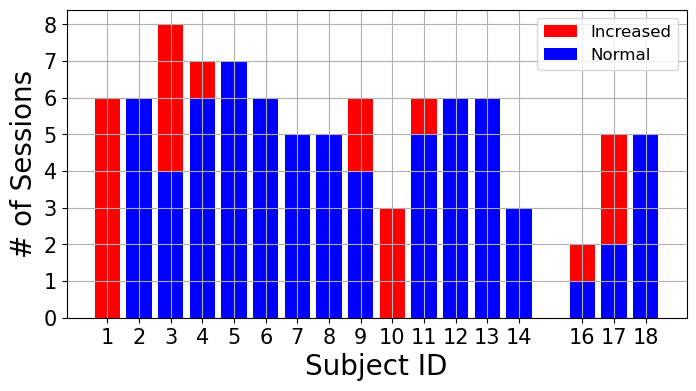
\includegraphics[width=1\linewidth]{figure/nb_sess_per_subject.png}
%     \caption[Number of sessions recorded from each subject.]{Number of sessions recorded from each subject. The elevated stress level sessions are indicated in red. The normal stress level sessions are indicated in blue.}
%     \label{nb_sess}
% \end{figure}

%%%%%%%%%%%%%%%%%%%%%%%%%%%%%%%%%%%%%%%%%%%%%%%%%%%%%%%%%%%%%%%%%%%%%
\subsubsection{Feature extraction}
Based on 50 frequency bins with a bin width of 1Hz, we estimated the power spectrum density (PSD) in the eye-open resting sessions.
To reduce the number of features, we selected frequency bins in the $\theta$ range as $\theta$ band activities have been linked to stress-related cognitive state changes in previous studies \cite{sani2014stress_detection_power, alonso2015stress_theta_increase}.
We did not analyze activities in frequency ranges because they overlapped with other non-brain artifacts, such as head movement \cite{goncharova2003emg_freq_range}, or did not reflect consistent stress-induced brain response.
% \st{Though some studies report ATTENUATION OF the power of $\alpha$ band decreases under EXPOSURE TO STRESSORS, we observed an increase instead. Hence, we did not cover $\alpha$ frequency range for feature extraction.}
% A detailed analysis is provided in Section \ref{cmpdata}.
% \st{We did not include $\beta$ and $\gamma$ bands because the frequency range is highly overlapped with muscle activities and can be unreliable in realistic scenarios.}
The final number of features used in the analysis was 150 (5 frequency bins $\times$ 30 channels).

%%%%%%%%%%%%%%%%%%%%%%%%%%%%%%%%%%%%%%%%%%%%%%%%%%%%%%%%%%%%%%%%%%%%%
\subsubsection{Synthetic minority over-sampling technique}
Training classifiers on the imbalanced classes can potentially bias results toward the majority group.
To alleviate the imbalanced classes problem, we evaluated the performance of the synthetic minority over-sampling technique (SMOTE) \cite{chawla2002smote}, which essentially interpolates data points in the smaller group to create balanced class sizes.
It does so by first randomly selecting one data point from the minority group.
Next, it calculates k-nearest neighbors in the minority group of the selected data point.
Finally, SMOTE randomly selects one neighbor and generates a synthetic minority data point between the selected data point and the neighbor.
By repeating this process, the number of data points in the majority and minority groups is equal.

%%%%%%%%%%%%%%%%%%%%%%%%%%%%%%%%%%%%%%%%%%%%%%%%%%%%%%%%%%%%%%%%%%%%%
\subsection{Model selection and evaluation}
%%%%%%%%%%%%%%%%%%%%%%%%%%%%%%%%%%%%%%%%%%%%%%%%%%%%%%%%%%%%%%%%%%%%%
\subsubsection{Linear Discriminant Analysis}
\label{lda_method}
The first classification model we investigated is Linear Discriminant Analysis (LDA) \cite{balakrishnama1998LDA}, 
which aims to find a linear combination of features to separate different classes into different distributions.
In this study, we implement LDA in \texttt{scikit-learn} \cite{scikit-learn}, a Python library, with equal prior probabilities for both classes.
Since LDA is sensitive to outliers \cite{buyukozturk2008lda_outlier}, we further selected 3Hz to 7Hz from Fz, FCz, and Cz channels out of 150 features to prevent potential outlier effects.
These channels lie along the mid-line of the scalp topology, and previous studies have shown that they typically capture activities closely associated with changes in cognitive states within the \(\theta\) range \cite{attallah2020frontal_electrode}.
% \textcolor{red}{We selected these 15 features because we observed significant difference between increased and normal group in the PSD analysis. We introduced the details of the PSD analysis results in the Section \ref{ch1_results}.}

%%%%%%%%%%%%%%%%%%%%%%%%%%%%%%%%%%%%%%%%%%%%%%%%%%%%%%%%%%%%%%%%%%%%%
\subsubsection{Neural Network}
Besides the linear classifier, we also investigated the performance of A non-linear classifier.
In particular, we built a 4-layer fully connected neural network (NN) using \texttt{pyTorch} \cite{NEURIPS2019_9015pytorch} and trained this NN using the features from all the recording channels.
% To compare the NN to the LDA model, we also built another 4-layers fully connected NN with different numbers of nodes in each layers and trained this NN using the same features as the LDA model (Fz, FCz, and Cz).
Fig.~\ref{nn_struct} depicts the architectures of the NN.
We used ReLU as an activation function between layers and a Sigmoid function at the output layers.
The number of training epochs is 1000, and the loss function for backpropagation is binary cross-entropy loss.
% \textcolor{red}{To maximize the learning ability of NN while prevent overfitting, we also evaluated the effect of  the early stopping technique by reducing the number of training epochs from 1000 to 200 CITE}.

\begin{figure}
    \centering
    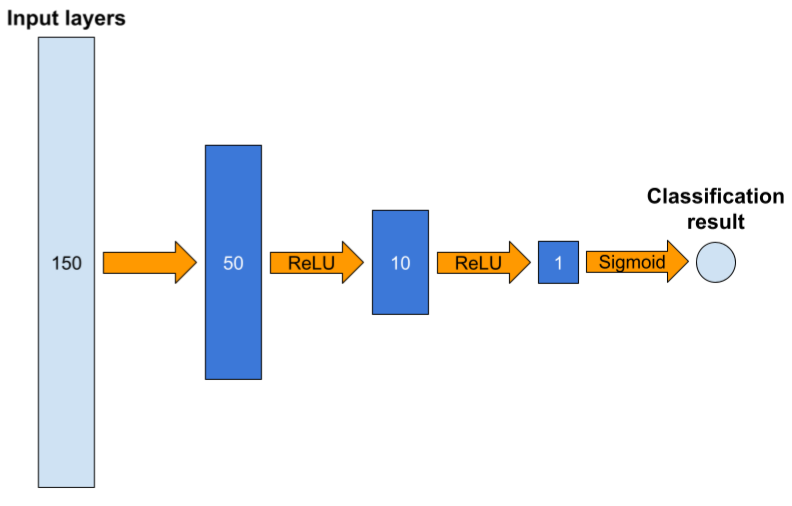
\includegraphics[width=1\linewidth]{figure/NN_struct_clip.png}
    \caption[The architecture of the Neural Network]{The architectures of the Neural Network used in this study. The number of nodes is indicated by the number in each layer. All the layers are fully connected to the next layer.}
    \label{nn_struct}
\end{figure}

%%%%%%%%%%%%%%%%%%%%%%%%%%%%%%%%%%%%%%%%%%%%%%%%%%%%%%%%%%%%%%%%%%%%%
\subsubsection{Model evaluation}
To evaluate the performance of our model, we implemented leave-one-session-out (LOO) cross-validation after model training.
LOO cross-validation selects a test session from the dataset and then trains the model on the rest of the sessions. Next, the trained model is applied to the test session. LOO cross-validation performs the same procedure for all sessions and finally reports the prediction results.
% \par
% Besides using leave-one-session-out validation to evaluate our model, we also performed leave-one-subject-out validation on the stress detection algorithms using LDA to evaluate if our models are biased to some specific subjects.
% Leave-one-subject-out validation has the same procedure as leave-one-session-out validation, except it picks out all the sessions from one subject per loop. The metrics of each loop were further summarized by mean operation.
\par
Since our dataset contains more normal than elevated stress sessions, the chance level calculated over all the sessions is 77.17\%.
Therefore, instead of using accuracy as a performance metric, we used balanced accuracy, which gives us a chance level of 0.5.
We also used the F1 Score to indicate the harmonic balance between recall and precision to characterize a model's sensitivity and specificity.

% \begin{equation}
%     \label{bas}
%     Balanced~Accuracy \;=\;\frac{1}{N_{class}}\sum^{N_{class}}_{i=1}~\frac{Number~of~correct~prediction~in~class~i}{Number~of~samples~in~class~i}https://www.overleaf.com/project/64e941964efe6de574ca83a4
% \end{equation}

% \begin{equation}
%     \label{f1}
%     F_1\;=\;2~\frac{precision\cdot recall}{precision+recall}
% \end{equation}

%%%%%%%%%%%%%%%%%%%%%%%%%%%%%%%%%%%%%%%%%%%%%%%%%%%%%%%%%%%%%%%%%%%%%
\subsection{Practical issues of deployment}
%%%%%%%%%%%%%%%%%%%%%%%%%%%%%%%%%%%%%%%%%%%%%%%%%%%%%%%%%%%%%%%%%%%%%
We must address several practical issues before deploying stress-detection systems in the real world.
First, we would like to monitor our stress levels in real time.
Unlike the laboratory scenarios, asking the users to wait 5 minutes before getting the results is unrealistic.
Hence, online capability is one of the most important indicators when we build our stress detection.
Second, we would like to reduce the number of recording channels needed in our stress detection because EEG setup can be time-consuming and labor-intensive.
Adding additional channels to a recording system may also increase its manufacturing cost significantly.
Therefore, we investigated the effect of recording channel reduction on our stress detection algorithms.

%%%%%%%%%%%%%%%%%%%%%%%%%%%%%%%%%%%%%%%%%%%%%%%%%%%%%%%%%%%%%%%%%%%%%
\subsubsection{Real-time ocular artifact removal}
Independent component analysis can identify artifact-related ICs, especially eye-related ICs, and remove them from the EEG signals \cite{Jung2000_bbs, bigdely2013eyecatch, Frolich2004}.
However, the computational time of ICA makes it unsuitable for real-time applications.
This study proposes an IC projection artifact removal method for removing eye-related artifacts without performing online ICA.
We focus solely on removing eye-related ICs for two key reasons. Firstly, eye activities introduce contamination into EEG signals within the frequency range of 0Hz to 8Hz, which coincides with the frequency band of our PSD features \cite{schlogl2007eog_freq_range}.
Second, compared to  sparse and complicated muscle activities, two kinds of the most severe eye artifacts, blink and horizontal saccade, can be well separated by ICA into blink- and saccade-related ICs.  Furthermore, these eye-related ICs exhibit remarkable similarity across subjects.
% as shown in Fig.~\ref{ex_rej_eye}. 
We performed ICA for each session separately to check whether most contained blink- and saccade-related ICs. We counted the number of eye-related ICs found in each session.
\par
Our proposed method is comprised of three steps.
First, we performed ICA on a single subject and recorded its ICA unmixing matrix $W$ and its ICA mixing matrix $W^{-1}$.
Next, we removed the blink- and saccade-related ICs from the mixing matrix $W^{-1}$ by assigning the corresponding columns to 0 and recorded this new mixing matrix $M^*$.
In cases where there is a discrepancy in the number of recording channels between the template and the processed data, we approximated the new mixing and unmixing matrices by retaining the rows in $M^*$ and the columns in $W$ according to the channel labels.
Finally, we combined the unmixing matrix and the new mixing matrix to create an IC decomposition template $P$.
This template can remove the eye-related IC activities using matrix multiplication, thereby preventing the need for online ICA execution.
% \par
% \mc{We compared the model performances trained on data preprocessed by the offline-ICA method and the proposed method.}
% \mc{We also evaluated whether the proposed method can maintain its performance when using a template recorded by 30 channels to process sessions recorded by 11 channels.}

 % \begin{align*}
 %     y\,&=\,Wx\\
 %     x\,&=\,W^{-1}Wx\\
 %     x_{without\,eye}\,&=\,M^*Wx\\
 %     x_{without\,eye}\,&=\,Px
 % \end{align*}

%%%%%%%%%%%%%%%%%%%%%%%%%%%%%%%%%%%%%%%%%%%%%%%%%%%%%%%%%%%%%%%%%%%%%
\subsubsection{Reduction of recording channels}
\label{sec_reduce_ch}
We compared three recording montages and their stress-detection performance to investigate the effect of recording channel reduction.
Besides the original 30 recording channels, we selected 11 and 5 channels in the frontal region out of the 30 channels.
Fig.~\ref{stress_ch} shows the location of the three channels.
We selected these channels because we would like to capture the eye-related ICs in the IC decomposition template.
After the channel reduction, we performed data preprocessing with the IC projection artifact removal method and trained our stress detection algorithms with LDA and NN.
One thing to clarify is that the number of nodes in the input layer of NN changes from 150 to 55 and 25, corresponding to 11 channels and 5 channels, to adapt to the change in the number of recording channels.

% sub select channel montage
\begin{figure}
    \centering
    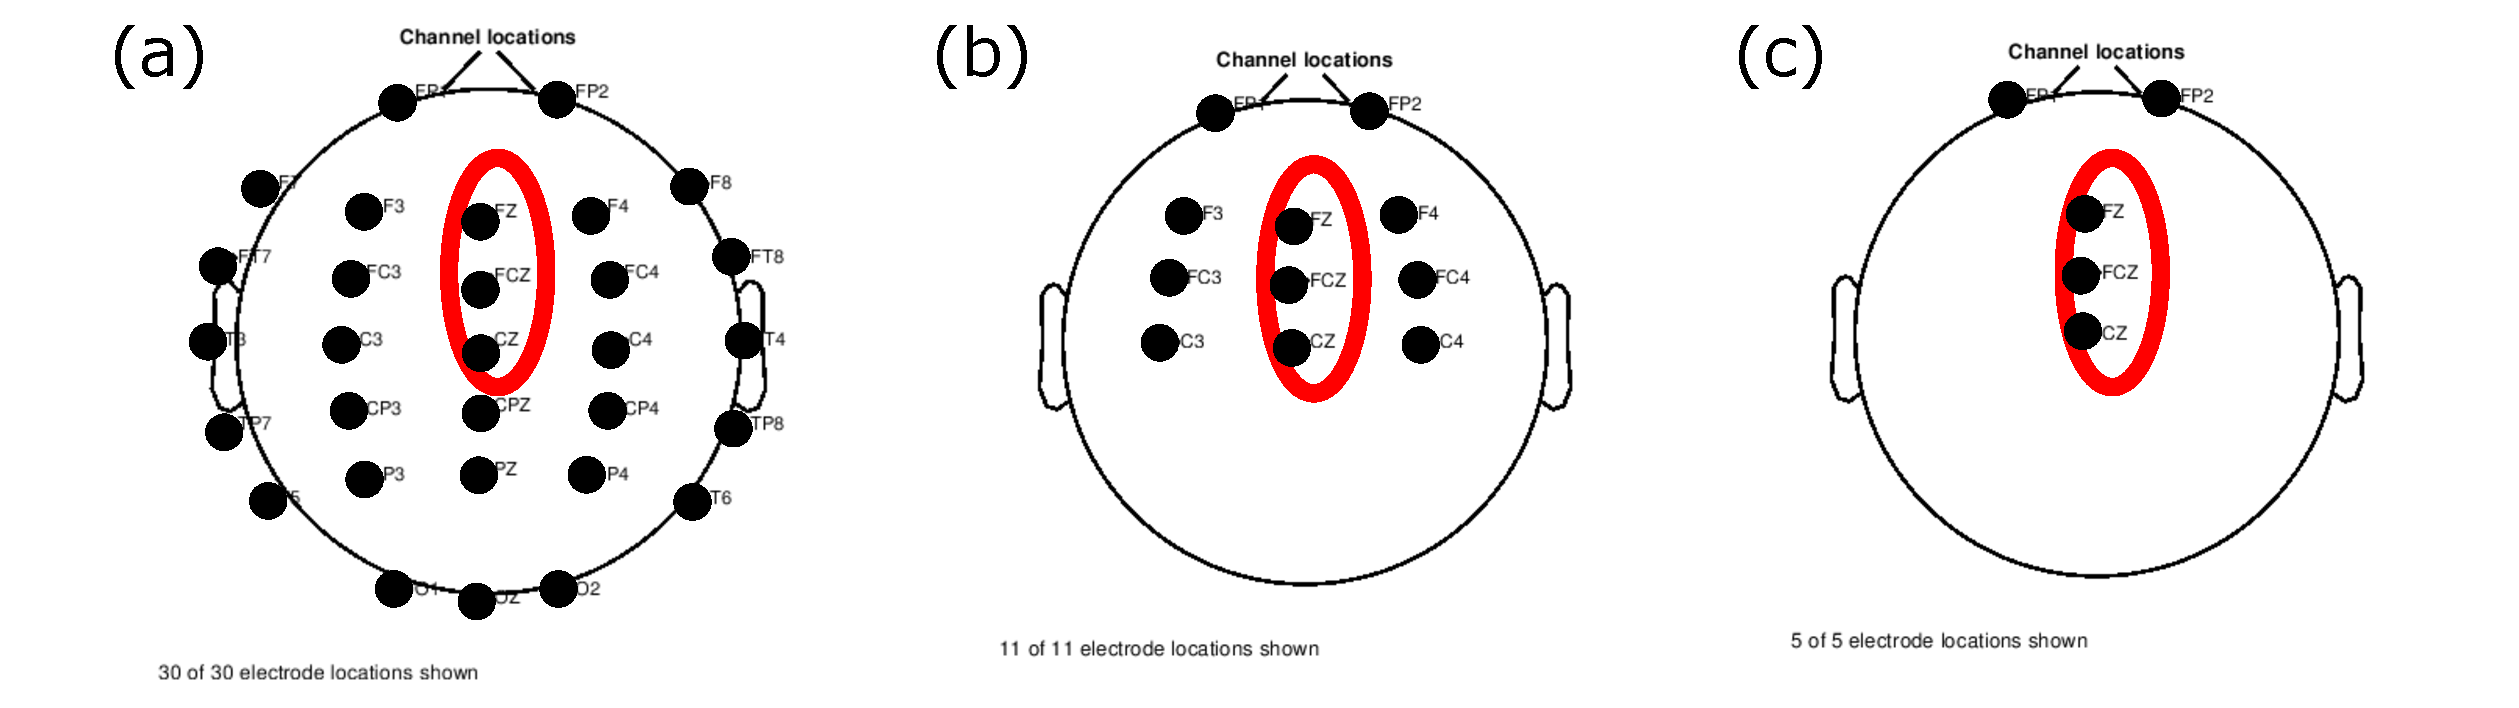
\includegraphics[width=1\linewidth]{figure/selectCh.pdf}
    \caption[Montage of channel reduction.]{Montage of channel reduction. (a) shows all 30 channels. (b) shows the subselected 11 channels. (c) shows the subselected 5 channels. The red circle indicates the location of 3 feature channels.}
    \label{stress_ch}
\end{figure}

%%%%%%%%%%%%%%%%%%%%%%%%%%%%%%%%%%%%%%%%%%%%%%%%%%%%%%%%%%%%%%%%%%%%%
\subsubsection{Online stress detection evaluation}
\label{sec_online_stress}
We investigated two important parameters in online use cases: the length of the sliding window for the PSD estimation and the step size to move the sliding window forward.
% To evaluate the relationship between the window length and the step size, we applied our LDA stress detection with different window lengths and step sizes.
First, we segmented a session into multiple epochs using different sliding window lengths and step sizes.
Next, we trained our LDA stress detection model using the rest of the sessions and applied the model to the epochs.
For each window, we had a prediction about whether the session was in the elevated stress group or the normal stress group.
To summarize these predictions, we used a majority vote to assign the session to the group with the most predictions.
After repeating this process for all the sessions, we calculated the balanced accuracy for each pair of sliding window lengths and step sizes.

%%%%%%%%%%%%%%%%%%%%%%%%%%%%%%%%%%%%%%%%%%%%%%%%%%%%%%%%%%%%%%%%%%%%%
\section{Results}
%%%%%%%%%%%%%%%%%%%%%%%%%%%%%%%%%%%%%%%%%%%%%%%%%%%%%%%%%%%%%%%%%%%%%
\subsection{Stress detection with and without artifact removal and SMOTE}
% \subsection{Stress detection with and without artifact removal}
% \label{cmpdata}
% Fig.~\ref{stress_cmpdata} SHOWS the RAW CHANNEL EEG \st{signals} before and after our artifact removal pipeline.
% AS ILLUSTRATED IN Fig.~\ref{stress_cmpdata} (a), \st{we can see there are several} eye blinks DISTORT the SIGNALS OVER the frontal region, and there is a BROADLY DISTRIBUTED muscle-related artifact caused by jaw clenching.
% BY CONTRAST, in Fig.~\ref{stress_cmpdata} (b), the eye blink DISTORTIONS have been removed by our artifact removal pipeline and the contamination from the jaw clenching has been diminished.

% data before and after artifact removal
% \begin{figure}
%      \centering
%      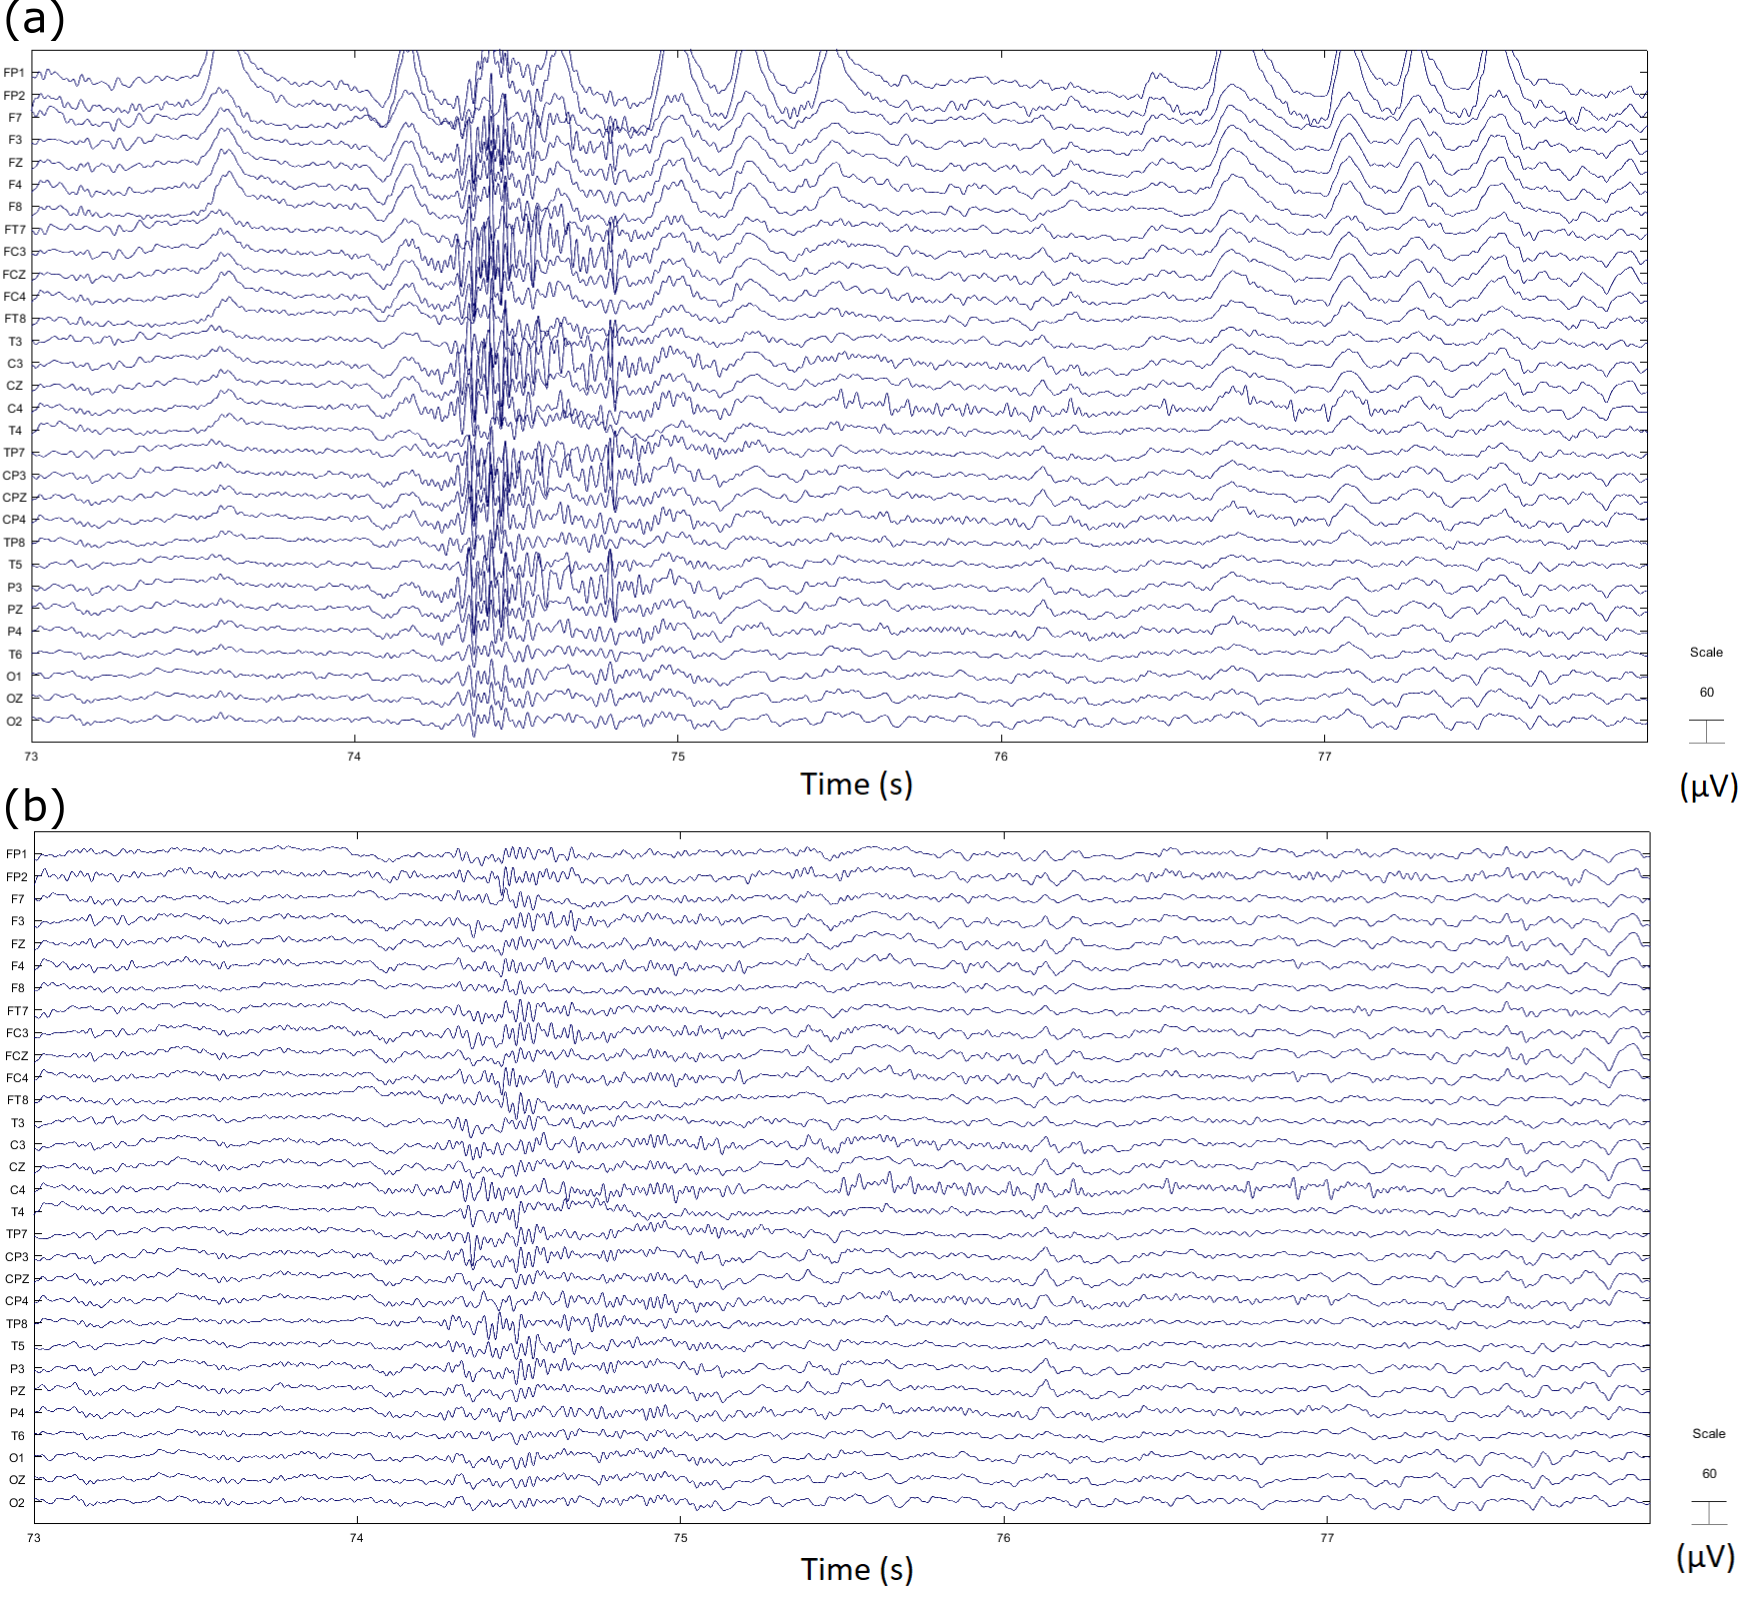
\includegraphics[width=1\linewidth]{figure/cmp_data.png}
%      \caption[Example of the performance of artifact removal]{Artifact removal APPLIED TO EEG. (a) shows the ORIGINAL % DATA AFTER bandpass FILTERING (b) shows the SAME data after applying our artifact removal pipeline.}
%      \label{stress_cmpdata}
% \end{figure}

Fig.~\ref{cmp_psd} shows the effect of our artifact-removal pipeline on the PSD features of selected channels.
On the top row, the PSDs of the elevated and normal stress groups  T after band-pass filtering alone do not directly differentiate in the feature frequency range of all the feature channels.
On the other hand, after artifact removal, we found noticeable group differences between 4 to 10Hz over all three channels (bottom row). The scale of the PSD also dropped from 20 dB to 10dB after artifact removal.

% % PSD before and after artifact removal
\begin{figure}
 	\centering
 	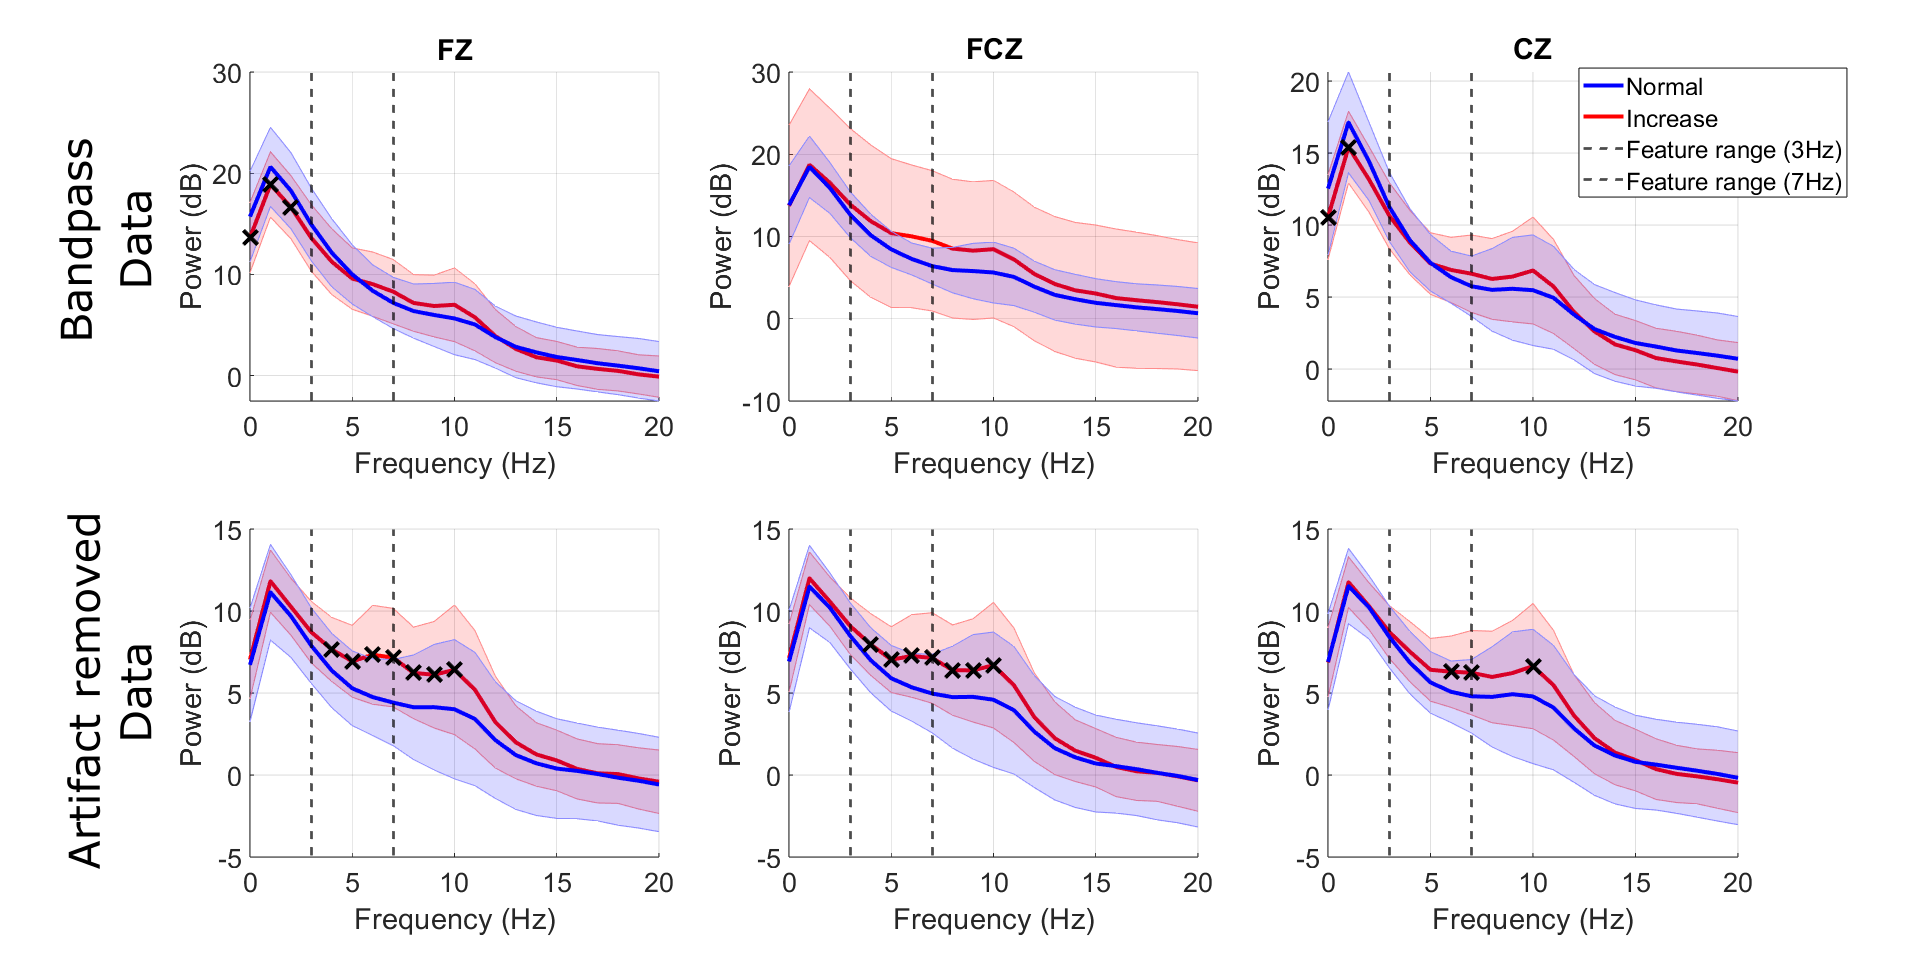
\includegraphics[width=1\linewidth]{figure/cmp_psd_new.png}
 	\caption[PSD features of selected channels before and after artifact removal]{PSD features of selected channels before and after artifact removal. The first row shows the PSDs of band-pass-filtered only data. The second row shows the PSDs of data that have undergone artifact removal. The spectral activities of the normal and elevated stress groups are shown in blue and red, respectively. The solid lines indicate the mean, and the shaded area indicates the standard deviation across sessions. The cross dots indicate frequency bins in which the spectral power of EEG activities reliably differentiates the two groups using a bootstrap test ($p<0.05$). The dashed line indicates the frequency range used in the LDA analysis.}
 	\label{cmp_psd}
\end{figure}

The comparisons of stress detection performance before and after artifact removal are shown in Table~\ref{stress_lda_artifact} and Table~\ref{stress_nn_artifact} concerning the LDA model and NN model.
In both models, we observe a gradual increase in accuracy and balanced accuracy after each artifact removal step.
Also, the performance of the LDA model is always better than the NN model.
The best performance appears when combining ASR with offline ICA.
When replacing the offline ICA method with the IC projection artifact removal method, we observe noticeable improvements compared to applying ASR alone in both models.
Moreover, there is only a 1\% difference between the LOO balanced accuracy of the proposed method and offline ICA in the LDA model.
 % Given the  Fig.~\ref{cmp_psd}, we also compared the performance of LDA stress detection with a fixed frequency range (3Hz to 7Hz) and significantly different frequency bins in each channel (shown as \st{a} crossES in Fig.~\ref{cmp_psd}) features.
% The balanced accuracy of using significantly different frequency bin features is 6\% worse than using the fixed frequency range features.
% To compare the two models, we trained our NN stress detection using the LDA features described in \ref{lda_method} with the architecture described in Fig.~\ref{nn_struct} (b).
% With the same features, the accuracy of NN 2\% worse than the accuracy of LDA and the balanced accuracy of NN is 18\% worse than the balanced accuracy of LDA.

% lda artifact removal table
\begin{table}[b]
\centering
\caption[The effects of artifact removal on LDA stress detection]{The effects of artifact removal on the performance of LDA-based stress detection. BP refers to band-pass filtering. Projection refers to the IC projection artifact removal method.}
\begin{tabular*}{\linewidth}{@{\extracolsep{\fill}} l|c c c}
    \specialrule{1.5pt}{0pt}{0pt}
    \multicolumn{1}{c|}{\textbf{LDA}}
    & \textbf{LOO Acc.}
    & \textbf{LOO Balanced Acc.}
    & \textbf{F1}
    \\
    \specialrule{1.5pt}{0pt}{0pt}
    BP Only
    & 68.48\%
    & 62.81\%
    & 0.43
    \\ \hline
    BP + ASR
    & 72.83\%
    & 70.66\%
    & 0.53
    \\ \hline
    \textbf{BP + ASR + ICA}
    & \textbf{79.35\%}
    & \textbf{78.24\%}
    & \textbf{0.63}
    \\ \hline
    BP + ASR + Projection
    & 80.43\%
    & 77.26\%
    & 0.63
    % \\ \hline
    % BP + ASR + ICA (sig. feat.)
    % & 78.26\%
    % & 72.50\%
    % & 0.57
    \\ \specialrule{1.5pt}{0pt}{0pt}
\end{tabular*}
\label{stress_lda_artifact}
\end{table}


% nn artifact removal table
\begin{table}[t]
\centering
\caption[The effects of artifact removal on 4-layer NN stress detection]{The effects of artifact removal on the performance of 4-layer NN stress detection. BP refers to band-pass filtering. Projection refers to the IC projection artifact removal method.}
\begin{tabular*}{\linewidth}{@{\extracolsep{\fill}} l|c c c}
    \specialrule{1.5pt}{0pt}{0pt}
    \multicolumn{1}{c|}{NN}
    & LOO Acc.
    & LOO Balanced Acc.
    & F1
    \\
    \specialrule{1.5pt}{0pt}{0pt}
    BP Only
    & 75.00\%
    & 56.98\%
    & 0.3
    \\ \hline
    BP + ASR
    & 77.17\%
    & 66.77\%
    & 0.49
    \\ \hline
    \textbf{BP + ASR + ICA}
    & \textbf{83.70\%}
    & \textbf{74.35\%}
    & \textbf{0.62}
    \\ \hline
    BP + ASR + Projection
    & 80.43\%
    & 68.88\%
    & 0.53
    % \\ \hline
    % BP + ASR + ICA (LDA features)
    % & 77.17\%
    % & 61.74\%
    % & 0.4
    \\
    \specialrule{1.5pt}{0pt}{0pt}
\end{tabular*}
\label{stress_nn_artifact}
\end{table}

Since our two groups of data did not contain balanced numbers of datasets, we evaluated whether SMOTE could enhance the performance of our stress detection models.
Table~\ref{stress_smote} shows the effect of SMOTE on the analysis after the artifact removal pipeline with offline ICA.
Though the LOO balanced accuracy increased slightly, there was no significant improvement in both models with the SMOTE process.
\par
In the following analysis, we only reported the results from the LDA model without SMOTE, as the LDA model consistently outperformed the NN model, and the effect of SMOTE was found to be negligible.
% In the following analysis, we only performed SMOTE on the NN stress detection algorithms because the ACCURACY improvement of LDA stress detection algorithms after SMOTE WAS less significant on the DATA THAT UNDERWENT ARTIFACT REMOVAL compared to the DATA THAT WAS BANDPASS FILTERED ONLY, as shown in Table \ref{stress_raw_results} (1\% improvement versus 5\% improvement).
% However, when we applied SMOTE TO the NN model trained with LDA features, the balanced accuracy ROSE from 61\% to 72\% -- which is close to the performance of the NN model trained with features from all recording channels (74\%).

% SMOTE table
\begin{table}[t]
\centering
\caption[The effects of SMOTE on LDA and NN stress detection]{The effect\st{s} of SMOTE on LDA and NN stress detection.}
\begin{tabular*}{\linewidth}{@{\extracolsep{\fill}} l|c c c}
    \specialrule{1.5pt}{0pt}{0pt}
    & LOO Acc.
    & LOO Balanced Acc.
    & F1
    \\
    \specialrule{1.5pt}{0pt}{0pt}
    LDA (w/o SMOTE)
    & 79.35\%
    & 78.24\%
    & 0.63
    \\ \hline
    LDA (w/ SMOTE)
    & 81.52\%
    & 79.64\%
    & 0.65
    \\ \hline
    NN (w/o SMOTE)
    & 83.70\%
    & 74.35\%
    & 0.62
    \\ \hline
    NN (w/ SMOTE)
    & 81.52\%
    & 76.29\%
    & 0.62
    % \\ \hline
    % NN (LDA features w/o SMOTE)
    % & 77.17\%
    % & 61.74\%
    % & 0.4
    % \\ \hline
    % NN (LDA features w/ SMOTE)
    % & 78.26\%
    % & 72.50\%
    % & 0.57
    \\
    \specialrule{1.5pt}{0pt}{0pt}
\end{tabular*}
\label{stress_smote}
\end{table}

%%%%%%%%%%%%%%%%%%%%%%%%%%%%%%%%%%%%%%%%%%%%%%%%%%%%%%%%%%%%%%%%%%%%%
\subsection{Consistency of eye-related ICs across different recordings}
To evaluate the consistency of eye-related ICs across different recordings, Figure.~\ref{nb_eyeIC_portion} shows the portion of sessions with different numbers of eye-related ICs found.
We found that 45.7\% of sessions contain two eye-related ICs, and 42.4\% of sessions contain three eye-related ICs.
Moreover, only 2.2\% of sessions contain no eye-related ICs.
Fig.~\ref{ex_3_eye} shows an example of the three eye-related ICs in a session.
% In this example, we once again observed blink-related IC and saccade-related IC.

% number of eye IC found in each session
\begin{figure}
    \centering
    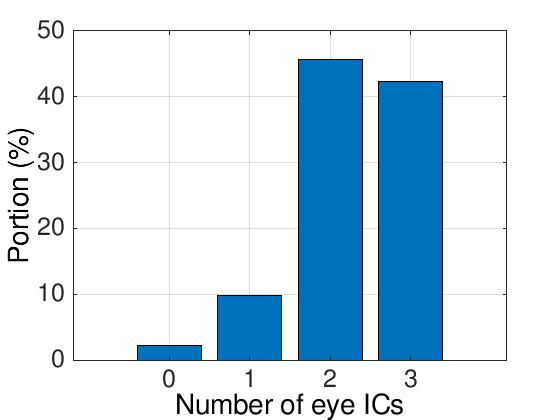
\includegraphics[width=0.7\linewidth]{figure/nb_eyeIC_portion.png}
    \caption[Histogram of the number of eye-related ICs found in each session.]{Histogram of the number of eye-related ICs found in each session. The histogram has been normalized by the number of sessions.}
    \label{nb_eyeIC_portion}
\end{figure}

% % example of 3 eye ICs
\begin{figure}
     \centering
     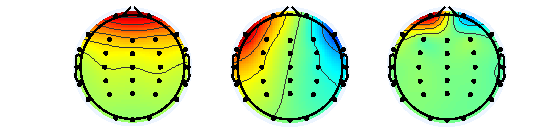
\includegraphics[width=0.8\linewidth]{figure/three_eyeIC_example.png}
     \caption[Example of the three eye-related ICs found within a session.]{Example of the three eye-related ICs found within a session. The left and center ICs correspond to blink- and saccade-related ICs, respectively.}
     \label{ex_3_eye}
 \end{figure}

 \begin{figure}
    \centering
    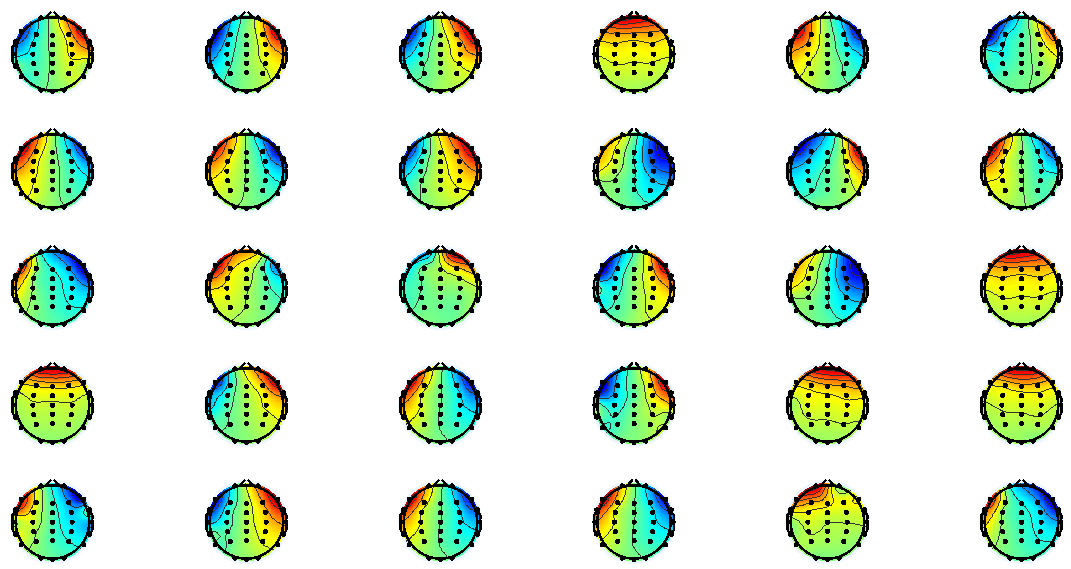
\includegraphics[width=1\linewidth]{figure/rej_eyeIC_example.png}
    \caption[Example of the rejected eye-related ICs.]{Example of the rejected eye-related ICs.}
    \label{ex_rej_eye}
\end{figure}

% Next, we examined whether we could apply the proposed method to a session recorded by a few recording channels using a template recorded by a higher amount of channels.
% Table \ref{cmp_proj_higher} compared the effect of using different templates on the performance of our LDA-based stress detection.

% We found \st{there are} a 13\% accuracy drop and an 18\% balanced accuracy drop in the 11-channels LDA-BASED stress detection ACCURACY WITH 11 CHANNELS after replacing the 11-channel\st{s} template with the truncated 30-channel template.

% % cmp project higher
% \begin{table*}[t]
% \centering
% \caption[The effect of different templates on the performance of LDA stress detection.]{\mc{The effect of different templates on the performance of LDA IN stress LEVEL CLASSIFICATION. BP refers to bandpass filtering. Proj. refers to our proposed IC projection method followed by the template used.}}
% \begin{tabular*}{\linewidth}{@{\extracolsep{\fill}} l|l c c c}
%     \hline
%     \multicolumn{1}{c|}{LDA}
%     & Preprocessing
%     & LOO Acc.
%     & LOO Balanced Acc.
%     & F1
%     \\ \hline
%     & BP Only
%     & 68.48\%
%     & 62.81\%
%     & 0.43
%     \\ \hline\hline
%     \multirow{2}{*}{30 Channels} & \multicolumn{1}{l}{BP+ASR+ICA} & \multicolumn{1}{c}{79.35\%} & \multicolumn{1}{c}{78.24\%} & \multicolumn{1}{c}{0.63} \\\cline{2-5}
%     & \multicolumn{1}{l}{Proj., 30-channels template} & \multicolumn{1}{c}{80.43\%} & \multicolumn{1}{c}{77.26\%} & \multicolumn{1}{c}{0.63} \\\hline\hline
%     \multirow{2}{*}{11 Channels} & \multicolumn{1}{l}{Proj., 11-channels template} & \multicolumn{1}{c}{80.43\%} & \multicolumn{1}{c}{78.94\%} & \multicolumn{1}{c}{0.64} \\\cline{2-5}
%     & \multicolumn{1}{l}{Proj., 30-channels template} & \multicolumn{1}{c}{63.04\%} & \multicolumn{1}{c}{60.97\%} & \multicolumn{1}{c}{0.41} 
%     \\ \hline
% \end{tabular*}
% \label{cmp_proj_higher}
% \end{table*}

%%%%%%%%%%%%%%%%%%%%%%%%%%%%%%%%%%%%%%%%%%%%%%%%%%%%%%%%%%%%%%%%%%%%%
\subsection{Effect of reducing the channel montage on stress level classification accuracy}
After evaluating the performance of the IC projection artifact removal method, we further compared the effect of reducing the number of recording channels.
Table~\ref{stress_lda_ch} shows the performance of the LDA models trained on data recorded by different input channels.
% Table~\ref{stress_lda_ch} and Table~\ref{stress_nn_ch} show the results of the LDA and NN models, respectively.
All data were processed using the IC projection artifact removal method before training LDA models.
We found that the performance of the LDA classifier increased by 1\% after the electrode montage was reduced from 30 to 11 channels.
However, with a 5-channel montage, the balanced accuracy dropped drastically from 77\% to 60\%.
% Table~\ref{stress_nn_ch} shows how the performance of the NN model gradually declined as the number of recording channels decreased.
% On the other hand, similar to the results of the LDA model, the performance of NN stress detection using LDA features WAS IMPACTED ONLY BY A VERY STEEP REDUCTION IN INPUT CHANNELS.  ACCURACY ACTUALLY increaseD BY 1\% THE CHANNEL MONTAGE WAS REDUCED FROM 30 to 11; HOWEVER, the balanced accuracy dropPED from 72\% to 54\% when WITH ONLY FIVE INPUT CHANNELS.

% lda channel table
\begin{table}[t]
\centering
\caption[The effects of channel reduction on LDA-based stress detection]{The effects of reducing input channels on the performance of LDA-based stress detection. After reducing the channel montage, the data are preprocessed using the proposed projection method. All the models used frequency bins between 3 to 7Hz on Fz, FCz, and Cz as features.}
\begin{tabular*}{\linewidth}{@{\extracolsep{\fill}} l|c c c}
    \specialrule{1.5pt}{0pt}{0pt}
    \multicolumn{1}{c|}{LDA}
    & LOO Acc.
    & LOO Balanced Acc.
    & F1
    \\
    \specialrule{1.5pt}{0pt}{0pt}
    30 Channels
    & 80.43\%
    & 77.26\%
    & 0.63
    \\ \hline
    \textbf{11 Channels}
    & \textbf{80.43\%}
    & \textbf{78.94\%}
    & \textbf{0.64}
    \\ \hline
    5 Channels
    & 67.39\%
    & 60.43\%
    & 0.40
    \\
    \specialrule{1.5pt}{0pt}{0pt}
\end{tabular*}
\label{stress_lda_ch}
\end{table}

% % NN channel table
% \begin{table}[t]
% \centering
% \caption[The effects of channel reduction on NN stress detection]{The reducing input channels on the performance of NN stress detection. After reducing the channel montage, the data are preprocessed using the proposed projection method. The sizes of the input layer in the NN models trained with features from all input channels are 150, 55, and 25 -- corresponding to the 30-channel, 11-channel, and 5-channel models, respectively. \mc{All models WERE preprocessed by SMOTE.}}
% \begin{tabular*}{\linewidth}{@{\extracolsep{\fill}} l|c c c}
%     \specialrule{1.5pt}{0pt}{0pt}
%     \multicolumn{1}{c|}{NN}
%     & LOO Acc.
%     & LOO Balanced Acc.
%     & F1
%     \\
%     \specialrule{1.5pt}{0pt}{0pt}
%     30-channel model
%     % & 83.70\%
%     % & 74.35\%
%     % & 0.62
%     & 78.26\%
%     & 67.47\%
%     & 0.50
%     \\ \hline
%     11-channel model
%     % & 77.17\%
%     % & 68.44\%
%     % & 0.51
%     & 75.00\%
%     & 65.36\%
%     & 0.47 
%     \\ \hline
%     5-channel model
%     % & 71.74\%
%     % & 59.89\%
%     % & 0.38
%     & 72.83\%
%     & 62.27\%
%     & 0.42
%     % \\ \hline
%     % LDA features, 30 channels
%     % & 78.26\%
%     % & 72.50\%
%     % & 0.57
%     % \\ \hline
%     % \textbf{LDA features, 11 channels}
%     % & \textbf{79.35\%}
%     % & \textbf{73.21\%}
%     % & \textbf{0.58}
%     % \\ \hline
%     % LDA features, 5 channels
%     % & 68.48\%
%     % & 54.43\%
%     % & 0.29
%     \\
%     \specialrule{1.5pt}{0pt}{0pt}
% \end{tabular*}
% \label{stress_nn_ch}
% \end{table}

% Fig.~\ref{eyeIC_example} shows an example of a template IC decomposition calculated from different numbers of recording channels.
% Fig.~\ref{eyeIC_example} (a) and (b) show that blink-related and saccade-related ICs, (inside the red squares) can be found in the template IC decompositions of 30 and 11 channels.
% However, there is no obvious eye-related IC in the template five-channel IC decomposition.

% % eye example
% \begin{figure}
%     \centering
%     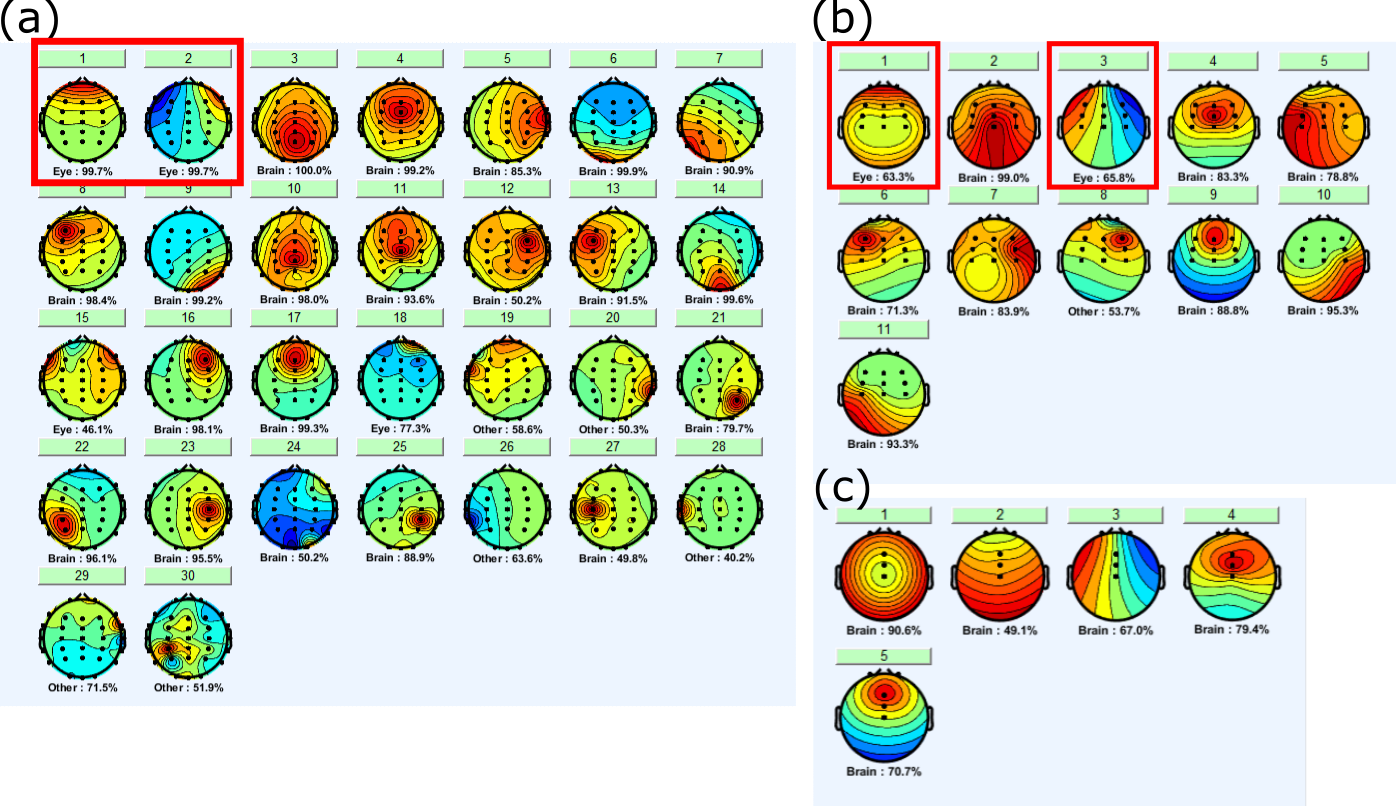
\includegraphics[width=1\linewidth]{figure/eyeIC_example.png}
%     \caption[Example of the IC decomposition template.]{Example of the IC decomposition template calculated from different numbers of recording channels. The components are classified by \texttt{ICLabel} and eye components for blink and saccade are marked by the red square.}
%     \label{eyeIC_example}
% \end{figure}

%%%%%%%%%%%%%%%%%%%%%%%%%%%%%%%%%%%%%%%%%%%%%%%%%%%%%%%%%%%%%%%%%%%%%
% \subsection{Subject variability}
% We summarized outcomes of the LDA model using different quantities of input channels and different preprocessing pipelines using leave-one-session-out validation and leave-one-subject-out validation in Table \ref{lo-session-o summary} and Table \ref{lo-subject-o summary}, respectively.
% \par
% To exclude any potential bias that could be caused by subjects with only one label, we selected only those subjects whose responses were assigned to both the normal \textit{and} elevated stress groups on different sessions and compared the balanced accuracy before and after artifact removal using 11 recording channels.
% We found that the balanced accuracy of Subjects 3, 4, and 9 was unchanged after artifact removal.
% Balanced accuracy after artifact removal actually increased for Subjects 11 and 17, while decreasing for subject 16.
% The mean of the balanced accuracy was 63.18\% before artifact removal and 76.37\% after. 

% \begin{figure}
%     \centering
%     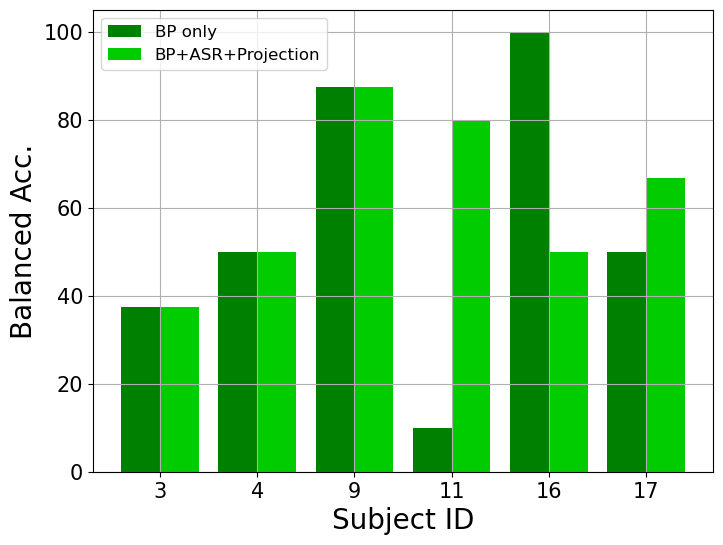
\includegraphics[width=\linewidth]{figure/cmp_bacc.png}
%     \caption[Balanced accuracy of each subject before and after artifact removal with 11 recording channels.]{Balanced accuracy of each subject before and after artifact removal using 11 recording channels. The figure only includes subjects with both normal and elevated stress. The dark green bars indicate the balanced accuracy before artifact removal. The light green bars indicate balanced accuracy after artifact removal.}
%     \label{cmp_bacc}
% \end{figure}

% lda loo session summary
\begin{table*}[t]
\centering
\caption[Leave-one-session-out validation of LDA stress detection]{Leave-one-session-out validation of LDA stress detection. All the models used frequency bins 3Hz to 7Hz on Fz, FCz, Cz as features. \textit{Proj}. refers to the IC projection artifact removal method.}
\begin{tabular*}{\textwidth}{@{\extracolsep{\fill}} l|l c c c}
    \specialrule{1.5pt}{0pt}{0pt}
    \multicolumn{1}{c|}{LDA}
    & Preprocessing
    & LOO Acc.
    & LOO Balanced Acc.
    & F1
    \\ \specialrule{1.5pt}{0pt}{0pt}
    & BP Only
    & 68.48\%
    & 62.81\%
    & 0.43
    \\ \hline\hline
    \multirow{3}{*}{30 Channels} & \multicolumn{1}{l}{BP+ASR} & \multicolumn{1}{c}{72.83\%} & \multicolumn{1}{c}{70.66\%} & \multicolumn{1}{c}{0.53} \\\cline{2-5}
    & \multicolumn{1}{l}{BP+ASR+ICA} & \multicolumn{1}{c}{79.35\%} & \multicolumn{1}{c}{78.24\%} & \multicolumn{1}{c}{0.63} \\\cline{2-5}
    & \multicolumn{1}{l}{BP+ASR+Proj.} & \multicolumn{1}{c}{80.43\%} & \multicolumn{1}{c}{77.26\%} & \multicolumn{1}{c}{0.63} \\\hline\hline
    \multirow{2}{*}{11 Channels} & \multicolumn{1}{l}{BP+ASR} & \multicolumn{1}{c}{75.00\%} & \multicolumn{1}{c}{75.42\%} & \multicolumn{1}{c}{0.58} \\\cline{2-5}
    & \multicolumn{1}{l}{\textbf{BP+ASR+Proj.}} & \multicolumn{1}{c}{\textbf{80.43\%}} & \multicolumn{1}{c}{\textbf{78.94\%}} & \multicolumn{1}{c}{\textbf{0.64}} \\\hline\hline
    \multirow{2}{*}{5 Channels} & \multicolumn{1}{l}{BP+ASR} & \multicolumn{1}{c}{70.65\%} & \multicolumn{1}{c}{64.22\%} & \multicolumn{1}{c}{0.45} \\\cline{2-5}
    & \multicolumn{1}{l}{BP+ASR+Proj.} & \multicolumn{1}{c}{67.39\%} & \multicolumn{1}{c}{60.43\%} & \multicolumn{1}{c}{0.40} 
    \\ \specialrule{1.5pt}{0pt}{0pt}
\end{tabular*}
\label{lo-session-o summary}
\end{table*}

% % lda loo subject summary
% \begin{table*}[t]
% \centering
% \caption[Leave-one-subject-out validation of LDA stress detection]{Leave-one-subject-out validation of LDA stress detection. All the models used frequency bins 3Hz to 7Hz on Fz, FCz, Cz as features. The mean operation is performed across all subjects. \textit{Proj}. refers to the IC projection artifact removal method.}
% \begin{tabular*}{\textwidth}{@{\extracolsep{\fill}} l|l c c }
%     \specialrule{1.5pt}{0pt}{0pt}
%     \multicolumn{1}{c|}{LDA}
%     & Preprocessing
%     & Mean Acc.
%     & Mean Balanced Acc.
%     \\ \specialrule{1.5pt}{0pt}{0pt}
%     & BP Only
%     & 64.84\%
%     & 63.18\%
%     \\ \hline\hline
%     \multirow{3}{*}{30 Channels} & \multicolumn{1}{l}{BP+ASR} & \multicolumn{1}{c}{68.17\%} & \multicolumn{1}{c}{66.51\%} \\\cline{2-4}
%     & \multicolumn{1}{l}{BP+ASR+ICA} & \multicolumn{1}{c}{72.63\%} & \multicolumn{1}{c}{72.93\%} \\\cline{2-4}
%     & \multicolumn{1}{l}{BP+ASR+Proj.} & \multicolumn{1}{c}{71.17\%} & \multicolumn{1}{c}{71.27\%} \\\hline\hline
%     \multirow{2}{*}{11 Channels} & \multicolumn{1}{l}{BP+ASR} & \multicolumn{1}{c}{71.35\%} & \multicolumn{1}{c}{71.95\%} \\\cline{2-4}
%     & \multicolumn{1}{l}{\textbf{BP+ASR+Proj.}} & \multicolumn{1}{c}{\textbf{77.05\%}} & \multicolumn{1}{c}{\textbf{76.37\%}} \\\hline\hline
%     \multirow{2}{*}{5 Channels} & \multicolumn{1}{l}{BP+ASR} & \multicolumn{1}{c}{62.07\%} & \multicolumn{1}{c}{61.19\%}\\\cline{2-4}
%     & \multicolumn{1}{l}{BP+ASR+Proj.} & \multicolumn{1}{c}{63.84\%} & \multicolumn{1}{c}{63.75\%}
%     \\ \specialrule{1.5pt}{0pt}{0pt}
% \end{tabular*}
% \label{lo-subject-o summary}
% \end{table*}

%%%%%%%%%%%%%%%%%%%%%%%%%%%%%%%%%%%%%%%%%%%%%%%%%%%%%%%%%%%%%%%%%%%%%
\subsection{Online stress detection}
We evaluate the online capability of our 11-channel LDA model with the IC projection artifact removal method.
We selected this model because of its potential to achieve comparable performance to the model processed by offline ICA with fewer recording channels.
Fig.~\ref{online_vote} shows the balanced accuracy of the 11-channel LDA model with different pairs of sliding window lengths and step sizes. 
When using a window length equal to 1 second, the balanced accuracy of the model hovers around 55\%. 
When the window length increases to 20 seconds, the balanced accuracy peaks at 78\%.
When the window length equals 5 minutes, the balanced accuracy drops to 75\%, and there is a 4\% decrease compared to offline results shown in Table~\ref{stress_lda_ch}.
Though the performance declined concomitantly with reductions in step sizes at window lengths of less than 20 seconds, we found that the difference in stress-detection performance with different step sizes was subtle, whereas the choice of window length dominated the model's performance.
Contrary to our expectations that a longer window length woudl provide better PSD estimation, the balanced accuracy actually declined when the window length is between 40 seconds and 3 minutes. 

\begin{figure*}
    \centering
    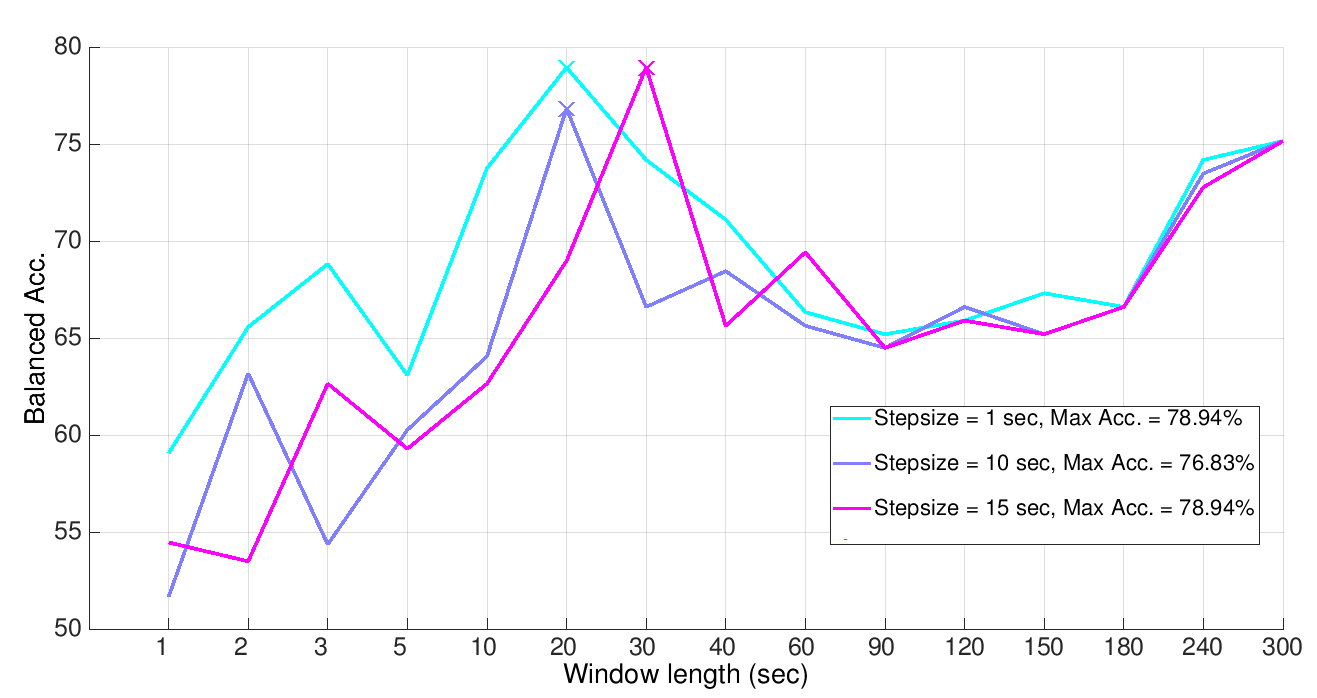
\includegraphics[width=1\linewidth]{figure/majority_vote_bacc_stepsize.png}
    \caption[Online evaluation with different window and step size]{Online evaluation with different windows and step sizes. Balanced accuracy is calculated from LOO results, and the prediction of each session is made by a majority vote across all the sliding windows. The cyan, blue, and purple lines show the results of step sizes 1 sec, 10 sec, and 15 sec, respectively. The window length with maximum balanced accuracy is marked by a cross in all step sizes.}
    \label{online_vote}
\end{figure*}

%%%%%%%%%%%%%%%%%%%%%%%%%%%%%%%%%%%%%%%%%%%%%%%%%%%%%%%%%%%%%%%%%%%%%
\section{Discussion}
%%%%%%%%%%%%%%%%%%%%%%%%%%%%%%%%%%%%%%%%%%%%%%%%%%%%%%%%%%%%%%%%%%%%%
Mental stress can greatly affect one's cognitive performance.
Detecting stress in daily life can benefit clinical treatments and task performance, as mental stress can impact many aspects of a person's cognitive and physiological functions.
However, stepping into the real world outside of a research lab's controlled conditions brings several challenges. 
In this study, we addressed the following considerations that are key to successful real-world stress detection: (1) obtaining robust EEG signal through artifact removal, (2) online classification capabilities using the IC projection artifact removal method, and (3) optimizing the number of input EEG channels.
% \par
% PSD
% The results show that our artifact removal pipeline can effectively remove artifacts INTRODUCED BY [ENUMERATE ARTIFACT TYPES HERE] (Fig.~\ref{stress_cmpdata}) and improve the CLASSIFICATION OF ELEVATED VERSUS NORMAL STRESS RESPONSES -- PARTICULARLY IN THE RANGE OF 3 TO 7 Hz OF THE EEG PSD (Table~\ref{stress_lda_artifact}, \ref{stress_nn_artifact}).
% \st{Since the artifacts have been removed, we can estimate the brain signals PSD more robustly and capture the significant difference in our PSD features between the increase and normal stress level groups, especially in the range of 3Hz to 7Hz.}
% Moreover, the scale of the PSD after artifact removal aligns with the empirical observations.
% We used a bootstrap statistical test\st{as our statistical test} because the number of sessions DIFFERED BETWEEN GROUPS, and the variances WITHIN each group WERE NOT EQUAL, especially for the PSD without artifact removal OVER FCz, as shown in Fig.~\ref{cmp_psd}.
\par
% stress detection after artifact removal
Each step in our artifact removal pipeline incrementally improved the performance of our stress detection models, as shown in Table~\ref{stress_lda_artifact} and Table \ref{stress_nn_artifact}.
Moreover, our proposed IC projection artifact removal method yielded a balanced accuracy comparable to offline ICA.
These results suggest that there is limited room for improvement in further removing muscle artifacts after removing eye artifacts.
% The comparable accuracy of the proposed method also suggest that eye-related ICs demonstrate consistency across subjects.
% These results indicate that contamination from eye artifacts is more severe than muscle artifacts in stress detection. 
% We also extractED \st{the significantly} different frequency bins for each channel as features as shown in Fig.~\ref{cmp_psd} and trained the LDA stress detection.
% However, the balanced accuracy of using these significantly different frequency bin features is worse than using the fixed frequency range features.
% We hypothesize that despite a reliable difference between spectral activities characterizing normal and elevated stress, the wide variance between 8Hz to 10Hz in both groups make LDA difficult to find a linear combination to minimize the within-group variance, thus leading to a reduction in accuracy.
\par
% validate our IC projection method
% 1. talk about eye portion, refer to fig. ex_eye and ex_muscle
Our proposed IC projection artifact removal method relies heavily on the consistency of eye-related ICs across recordings.
% Results in Fig.~\ref{ex_rej_eye} support the consistency of eye-related ICs, as the ICs can be approximately categorized into classes of either blink-related ICs or saccade-related ICs based on visual inspection.
Fig.~\ref{nb_eyeIC_portion} shows that nearly 90\% of the sessions in this dataset contain 2 or more eye-related ICs, indicating that blink-related and saccade-related ICs appear in almost all sessions.

In addition to identifying blink-related and saccade-related ICs, we observed an extra IC in certain sessions that could potentially be linked to minor lateral eye movements or facial expressions such as frowning. Conversely, the ICs associated with muscle activity exhibited greater diversity. Due to the complex nature of muscles, comprising numerous fibers, capturing a single body movement within a single IC poses a challenge for ICA.
%In addition, the signals generated by muscles have greater power %than the signals generated by the brain, resulting in extra demands %for ICs to explain muscle activities.

% \par
% explain why projection from higher number of channels don't work
% There are two problems that required further investigation on this method.
% First, we ASSUMED that the IC decomposition template WAS consistent across DIFFERENT datasets FROM A GIVEN PARTICIPANT -- and THUS, COULD be calculated from ANY SESSION OF DATA OBTAINED FROM A GIVEN INDVIDUAL.
% However, we DID NOT validate\st{d} this ASSUMPTION using other datasets.
% SecondLY, we BEGAN WITH THE PREMISE THAT the proposed method COULD be applied to A DATASET CONTAINING FEWER CHANNELS OF DATA THAN THE TEMPLATE. \st{with several recording channels less than the template's and larger than 2.}
% Since the proposed method is a component-based artifact removal method, A MINIMUM OF TWO components (AND HENCE TWO CHANNELS) ARE NEEDED to explain blinkS and saccadeS independently.
% Nevertheless, when we applied a 30-channel template TO 11-CHANNEL data, the ACCURACY OF OUR STRESS DETECTION MODELS DECLINED.
% One possible reason FOR THIS UNANTICIPATED OUTCOME is the approximation error caused by truncating the mixing and unmixing matriCES.
% The negative influence becomes INCREASINGLY severe as the difference between the template and the number of recording channels increase (SEE Table~\ref{cmp_proj_higher}).

\par
% compare LDA and NN
When comparing the performance of the LDA and NN models, we consistently observe superior performance from the LDA model over the NN model. One plausible explanation for this difference is overfitting. The NN model offers many trainable parameters, yet the available training data is relatively limited. Upon comparing models' performances with and without SMOTE, we noted only marginal enhancements for both LDA and NN models when employing SMOTE. This could be attributed to the scarcity of training data, as SMOTE assumes that the sampled data shares similar statistical characteristics with the underlying population.
% When training the NN model with LDA features without SMOTE, we \st{can} observeD high accuracy with low balanced accuracy, indicating THAT the model is strongly biased to the normal stress \st{level} group due to the imbalanced classes problem.
% With SMOTE procedure, the balanced accuracy of the NN model trained with the LDA features increased to the level of the balanced accuracy of the NN model trained with features from all channels.
% This result indicates that the selected channels (Fz, FCz, and Cz) contained most of the information related to cortical responses indicative of changes in subjective stress. 
% However, even with the improvement after SMOTE, the balanced accuracy of the NN model still fell behind that of the LDA model.

% \par
% One possible explanation for THE DECREASED BENEFIT OF SMOTE FOR LDA is that the features of the bandpass filtered data in feature space are relatively sparse compared to the FEATURES OF THE DATA THAT UNDERWENT ARTIFACT REMOVAL, and thus can benefit more from SMOTE on feature distribution estimation.
% Because the features of the DATA THAT UNDERWENT ARTIFACT REMOVAL are already condensed, the benefit of SMOTE on distribution estimation becomes less significant.

\par
% reduction of channel LDA
Low-density channel arrays are preferred to reduce setup times and equipment costs. 
Since ICA can decompose eye activities with channels near the frontal region, a full scalp montage may be unnecessary, particularly when using the proposed IC projection artifact removal method.
Moreover, our LDA model achieved comparable accuracy using only 11 versus 30 channels of EEG data (Table \ref{stress_lda_ch}), in keeping with the idea that features from a limited subset of channels (Fz, FCz, and Cz) can capture the discriminative information for reliable stress detection.
However, because our IC projection artifact removal method is based on independent components, its performance drops with too few input channels—as shown by our finding that with only 5 channels, ICA fails to decompose eye activities into distinct blink- and saccade-related ICs.
Instead, ICs represent a mixture of brain and eye activities.
Assuming that the most likely blink- and saccade-related ICs would be removed from the analysis, only three ICs would remain to reconstruct the surface EEG signals.
Also, a substantial portion of brain signals would be lost with the "mixed" ICs accounting for eye activities, resulting in a decline in model performance.
% We can clearly see the decline in model performance when using only 5 recording channels (Table \ref{stress_lda_ch}).
% \par
% % reduction of channel NN
% WE FOUND THAT USING LDA FEATURES LED TO BETTER PERFORMANCE OF THE NN MODEL COMPARED TO USING features from all the recording channels.
% This result indicates that OUR channel selection captureD the information related to stress level changes and preventED NN models from learning FEATURES OF THE brain signal THAT WERE irrelevant to stress level changes.
% On the other hand, when using 5 recording channels, the performance of NN stress detection with LDA features WAS worse than with features from all 5 recording channels because the NN stress detection with LDA features further removed the brain-related information from the already IMPOVERISHED signals by selecting 3 channels.
% \par
% % subject variability
% One concern of our stress detection algorithms is that they might reflect differences in the EEG signal driven by variability between participants rather than changes in stress-related arousal.
% To examine this concern, we first compared the leave-one-session-out validation and leave-one-subject-out validation results of our LDA stress detection algorithms.
% In both validations, the performance of the LDA model increased after each step in our artifact removal pipeline when using 11 and 30 recording channels while the performance decreased when using 5 recording channels.
% The agreement of results from two types of validation indicates that our stress detection captures stress-related arousal rather than subject variability.
% While the parallels between the leave-one-session-out and leave-one-subject-out validations are encouraging, we also undertook to investigate the balanced accuracy of the subjects with both elevated and normal stress sessions in the leave-one-subject-out validation.
% Though the balanced accuracy did not change for half of the subjects with both normal and elevated stress sessions, we found that in the other half, it increased for more subjects than decreased.
% % , and the mean of the balanced accuracy across subjects also increased after artifact removal.
% Moreover, the mean balanced accuracy after artifact removal was comparable to the leave-one-session-out balanced accuracy (76.39\% versus 78.94\%).
% These results support the notion that our classifications were based on stress level rather than subject variability.

\par
% window length and stepsize
Finally, we evaluated the online capability of the 11-channel LDA model with the IC projection artifact removal method by investigating the effect of different pairs of sliding window lengths and step sizes on the balanced accuracy.
The choice of window length over step size dominates the model's performance, probably because of the quality of the PSD estimation.
The longer the window length, the better the estimation quality.
We observed the best performances across different step sizes using a window length of around 20 seconds, indicating that the quality of PSD estimation was sufficient to detect stress level changes.
When the window length was shorter than the step size, the algorithm ignored the data points between them, resulting in a down-sampling effect that hampered the performance of stress detection.
The effect is more severe when using a large step size, as observed in Fig.~\ref{online_vote}.
On the other hand, at a window length of 5 minutes, we found that the balanced accuracy dropped slightly compared to the offline results, possibly because some sessions involved an eyes-open resting baseline that exceeds 5 minutes. 
\par
One thing that caught our attention is that, instead of a monotonic increase, the model's balanced accuracy dropped before returning to expected performance levels when using a 5-minute window length.
We hypothesize that mental stress changes do not affect EEG signals constantly, but rather, on a repeated cycle such that EEG-based changes due to psychological stress might be diluted by the long window length.
However, obtaining the benchmarks for stress detection in an online scenario would make testing this hypothesis very difficult.

%%%%%%%%%%%%%%%%%%%%%%%%%%%%%%%%%%%%%%%%%%%%%%%%%%%%%%%%%%%%%%%%%%%%%
\section{Conclusion}
This study proposes a robust, online capable, EEG-Based mental stress detection algorithm suitable for pervasive, real-world monitoring using a low-density channel array.
% We found that after our artifact removal pipeline, the PSD WAS significantly higher in the ELEVATED stress SESSIONS BETWEEN 4 TO 10 Hz OVER THE MIDLINE CHANNELS, Fz, FCz, and Cz.
To remove ocular artifacts in real time, we proposed an IC projection artifact removal method that reduced the required computational time while maintaining performance compared to offline ICA.
This study also explored the influence of different models, preprocessing pipelines, and the number of recording channels.
Our results show that with 15 features from Fz, FCz, and Cz channels, the proposed LDA-based stress detection algorithm can achieve a 78\% balanced accuracy in an imbalanced binary stress detection problem.
Moreover, for the purposes of artifact removal, the proposed LDA-based stress detection algorithm requires only 11 recording channels near the frontal region.
The findings of this study could lead to the deployment of daily mental stress monitoring in the future. 

%%%%%%%%%%%%%%%%%%%%%%%%%%%%%%%%%%%%%%%%%%%%%%%%%%%%%%%%%%%%%%%%%%%%%
\section{Acknowledgement}
Dr. Li-Wei Ko recorded the dataset used in this study at National Chiao Tung University (National Yang-Ming Chiao Tung University), Hsinchu, Taiwan.
The authors gratefully acknowledge the support from Dr. Li-Wei Ko, Microsoft Research, and the National Science Foundation.

% \addtolength{\textheight}{-13cm} 
%%%%%%%%%%%%%%%%%%%%%%%%%%%%%%%%%%%%%%%%%%%%%%%%%%%%%%%%%%%%%%%%%%%%%%%%%%%%%%%%

\bibliographystyle{IEEEtran}
\bibliography{bib_EMBC2018}
% \clearpage

% %%%%%%%%%%%%%%%%%%%%%%%%%%%%%%%%%%%%%%%%%%%%%%%%%%%%%%%%%%%
% \begin{IEEEbiography}[{\includegraphics[width=1in,height=1.25in,clip,keepaspectratio]{Chiyuan_profile_pic.jpg}}]{Chi-Yuan Chang}
% received the B.S. degree in mechanical engineering from the National Taiwan University, Taipei, Taiwan, in 2014. He is currently a Ph.D. student in Bioengineering from University of California, San Diego while at the Swartz Center for Computational Neuroscience. His major research interests include signal processing, robotics, and brain-computer interfaces.
% \end{IEEEbiography}

% \begin{IEEEbiography}[{\includegraphics[width=1in,height=1.25in,clip,keepaspectratio]{Shawn_profile_pic.png}}]{Sheng-Hsiou Hsu}
% (S’14) received the B.S. degree
% in electrical engineering from the National Taiwan University, Taipei, Taiwan, in 2011. He was a sole recipient of the scholarship of government sponsorship for overseas study in Biomedical Engineering in 2012. He received Ph.D. (2018) degrees in Bioengineering from University of California, San Diego while at the Swartz Center for Computational Neuroscience. His major research interests include brain-computer interfaces, machine learning, and signal processing with respect to functional imaging of brain dynamics.
% \end{IEEEbiography}

% \begin{IEEEbiography}[{\includegraphics[width=1in,height=1.25in,clip,keepaspectratio]{Luca_profile_pic.jpg}}]{Luca Pion-Tonachini}
% Luca Pion-Tonachini received the B.S. and M.S. degrees in electrical engineering with a focus in intelligent systems from the University of California San Diego (UCSD) in 2011 and 2014, respectively. He is currently pursuing the Ph.D. degree in electrical engineering, also at UCSD. As part of his doctoral program, he works at the Swartz Center for Computation Neuroscience (SCCN) developing tools for EEG processing and analysis using crowd labeling, deep neural networks, and semi-supervised machine learning and is also directly involved in efforts toward real-time artifact rejection and brain-state monitoring.
% \end{IEEEbiography}

% \begin{IEEEbiography}[{\includegraphics[width=1in,height=1.25in,clip,keepaspectratio]{TP_profile_pic.jpg}}]{Tzyy-Ping Jung}
% (F15) received the B.S. degree in electronics engineering from National Chiao Tung
% University, Hsinchu, Taiwan, in 1984, and the M.S. and Ph.D. degrees in electrical engineering from The Ohio State University, Columbus, OH, USA, in 1989 and 1993, respectively. He is currently a Research Scientist and the Co-Director of the Center for Advanced Neurological Engineering, Institute of Engineering in Medicine, University of California- San Diego (UCSD), La Jolla, CA, USA. He is also an Associate Director of the Swartz Center for Computational Neuroscience, Institute for Neural Computation, and an Adjunct Professor of Bioengineering at UCSD. In addition, he is an Adjunct Professor of Computer Science at the National Chiao Tung University, Hsinchu, Taiwan. He is also an Adjunct Professor at Tianjin University in China. His research interests are in the areas of biomedical signal processing, cognitive neuroscience, machine learning, time-frequency analysis of human EEG, functional neuroimaging, and brain-computer interfaces and interactions. 
% \end{IEEEbiography}

\end{document} 